\documentclass[12pt, a4paper   , oneside]{article}


\usepackage{fullpage}

\usepackage{setspace}
\onehalfspacing


\usepackage{epigraph}   % make nice quotes

\usepackage[export]{adjustbox}

\usepackage[osf,sc]{mathpazo}% Use the Palatino font
\usepackage[USenglish]{babel}
\usepackage{microtype} % Slightly tweak font spacing for aesthetics

\usepackage{titlesec} % Allows customization of titles
\titleformat{\section}[block]{\large\scshape\centering}{\thesection.}{1em}{} % Change the look of the section titles
\titleformat{\subsection}[block]{\large}{\thesubsection.}{1em}{} % Change the look of the section titles
\titleformat{\subsubsection}[block]{}{\thesubsubsection.}{1em}{} % Change the look of the section titles

\usepackage{fancyhdr} % Headers and footers


\usepackage{color}			% so you can have colors
\usepackage[gen]{eurosym}	% so you can use the Euro symbol \euro, gen option makes it look nicer, looks weird otherwise
\usepackage{verbatim}		% use \begin{verbatim} in order to have text instead of latex special characters = print source code without format


\usepackage[none]{hyphenat} % no hyphenation (=Silbentrennung)
\sloppy 					% words go over end of row without this
\usepackage{graphicx} 		% so that you can include graphics in the 
							% take care! if you use .pdf with \includegraphics, you can only compile with pdflatex
\usepackage[justification=centering]{caption}	% center captions of figures if the caption is longer than one line. 

\usepackage{subcaption}				% Create subfigures


%%% Math stuff
\usepackage{amsmath}				% Write more sophisticated formulas \begin{align}, \begin{eqnarray}
\usepackage{amssymb}                %features q.e.d. symbol
\usepackage{mathtools, nccmath}     %smaller equations in align environment

\allowdisplaybreaks

\usepackage{accents}

%%% Tables
\usepackage{booktabs}				% you need this to create tables from excel
\usepackage{longtable}				% needed for tables that are longer than 1 page --> \longtable instead of \tabular
									% also: dont create figure/table environment around longtable (figure environment creates box around it and then it doesnt work), also no centering!
\newcommand{\tablescale}{0.80}		% scale all tables according to that number: add \scalebox{\tablescale}{"contents"} around each table
									% scalebox command does not like captions -->make minipage environment, then caption+tabular in minipage environment, scalebox the minipage environment
									% add \footnotesize before notes -->notes are smaller
\usepackage{array}					% you can define new types of columns (not only l c r) for tables with \newcolumntype
									% Example: >{hsome declarationsi}{c}<{hsome more declarationsi}: \newcolumntype{x}{>{$}c<{$}} = column in math mode

						
\usepackage{multirow} 					% needed for tables so you can join rows
\usepackage{caption}					% needed to make table caption "Table 1" bold
\captionsetup[table]{labelfont=bf} 		% same as above
%\renewcommand\thetable{\Roman{table}} 	% Tables are enumerated with Roman numerals

\captionsetup[figure]{labelfont=bf} 

\usepackage{float}              %can use [H] to force latex to display tables/graphs at specified line
\usepackage{tikz,pgfplots,tikzscale}  
\usetikzlibrary{arrows, arrows.meta} %Create Graphs in Latex
\usetikzlibrary{shapes}
\usetikzlibrary{scopes}
\tikzset{every cross out node/.append style={-, solid}}
  \usepackage[font={small,it}]{caption}
%%% Bibliography
\usepackage[round]{natbib} 		%change citation style from [1] to Author(Year) by using \citet command (cite text), use round option to have round parenthesis
								% when citation is in parenthesis: \citep[before citation][after citation]{reference}, example: \citep[For instance][propose a model]{acharya_2014}
								% also: \citealp
%\bibliographystyle{plainnat} 	% choose style of bibliography of natbib package, {plainnat} is standard

%%% Weblinks und references
\usepackage[hidelinks]{hyperref}	% use \hyperlink{<Ziel>}{<Eingefasster Text>} setzt einen Link innerhalb eines Dokumentes. Das Ziel des Links wird mittels des Befehls \hypertarget{}{} festgelegt.
									% Fuer Ziele im WWW verwenden Sie bitte den Befehl \href{}{}.
									% hidelinks option: no ugly boxes around links and references. Links and references still clickable
									% also use \url{content}
\usepackage{xurl}

\hypersetup{colorlinks,citecolor=blue, linkcolor = blue, urlcolor  = blue} % Zitationen blau machen (linkcolor), "interne Verweise" (Fussnoten, Referenzen auf Sections/Bilder) blau machen(linkcolor) 
                                    
									
%%% Layout
%\usepackage{showframe}							% show margins
\setlength{\parskip}{5pt plus 2pt minus 1pt}	% Make some space after paragraph		

\makeatletter									% If there is a single figure or table on one page, 
\setlength{\@fptop}{0pt}						% the figure will be in the middle
\makeatother									% these options prevent that! figure will be on top

\frenchspacing									% Prevent double space between sentences (i.e. if you write ".", latex makes double instead of one space)
\interfootnotelinepenalty=10000

\newenvironment{tightcenter}{%
  \setlength\topsep{0pt}
  \setlength\parskip{0pt}
  \begin{center}
}{%
  \end{center}
}


\begin{document}


	
	\title{Capital Controls and the Global Financial Cycle\thanks{We thank 	Paul Bergin,  R. Anton Braun,  Nicolas Caramp, Andr\'{e}s Carvajal, Catherine Co, Athanasios Geromichalos, Karel Mertens,    Pablo Ottonello,  Alan M. Taylor, and Martín Uribe for valuable comments on the paper. We also thank Evi Pappa, an associate editor, and two anonymous referees for their guidance throughout the publication process. The  views  expressed  in  this  paper are  those  of  the  authors  and  do  not  necessarily  represent  those  of  the  Federal  Reserve  Bank  of Kansas  City  or  the  Federal  Reserve  System.}}
 		\author{Marina Lovchikova\footnote{E-mail: marina.lovchikova@gmail.com} \\ Covered California
		\and	 Johannes Matschke\footnote{Corresponding author, E-mail:Johannes.Matschke@kc.frb.org} \\ Federal Reserve Bank of Kansas City} 
		
		 %use \and to concatenate authors 
	%\date{\today}
	\date{} % No date on titlepage, if date not defined at all, automatically date=today
	\maketitle	
	\thispagestyle{empty}		% page does not have pagenumber
	\addtocounter{page}{-1}		% titlepage is not included in counter
	
		\begin{center}

	\today
	\end{center}
	
		\vspace{0.5cm}
		
	\begin{itshape} % Abstract starts here
		\begin{center}
			\textbf{Abstract}
		\end{center}
	\end{itshape}
		\noindent	% no tab before paragraph


Capital flows into emerging markets are volatile and risky, which sparked interest in active capital flow management. We first revisit the use of capital controls and discover a new stylized fact: Emerging markets, which actively revaluate their capital flow restrictions, increase  capital inflow controls during episodes of major international financial distress when investors are very risk averse and markets  volatile. We then explore this finding theoretically. We argue that heightened international financial volatility and investor risk aversion incentivize   regulators to reduce the amount of risky emerging market debt to cope with elevated risk premiums. This rationale can be decentralized via capital inflow restrictions during periods of major financial distress, consistent with the empirical findings. The paper hence provides an alternative to the familiar macroprudential motivation for capital controls.


	
		


	\vfill		%put Keywords and JEL at bottom of page (vfill: fill rest of page with empty space)
	

	\begin{description}
		
		\item \textbf{Keywords}: Capital Controls; Risk Aversion; Volatility; Risk Premium 
		\item \textbf{JEL: F36, F38, F41 } 
	\end{description}
	%%TC:endignore
	\newpage
	

	
\section{Introduction} \label{sec:intro}




The financial integration of emerging markets  has rekindled a debate on the advantages and disadvantages of international financial flows. Although foreign capital has   widely recognized benefits, sudden stops in capital flows may have lasting negative effects on macroeconomic and financial stability. The International Monetary Fund (IMF) shares this view and advocates for using capital controls under certain circumstances to address international capital surges (\citealp{ostry_2010}; \citealp{ostry_2011}).\footnote{The IMF  broadened its support for capital controls in 2022: \url{https://www.imf.org/en/Blogs/Articles/2022/03/30/blog033122-why-the-imf-is-updating-its-view-on-capital-flows}. Date accessed: 1/2/2024.} The IMF's  proposal is supported by a  theoretical literature which stresses that emerging markets borrow excessively in primarily foreign currency, which can generate vicious spirals of exchange rate depreciation and further tightening borrowing constraints (see, for example, \citealp{bianchi_2011}). The common policy prescription is then to impose macroprudential capital controls,  that is, to tighten restrictions when the economy is at risk prior to a potential sudden stop.\footnote{This does not imply that macroprudential capital controls are counter-cyclical. The risk of sudden stops, or a binding borrowing constraint, is largest immediately preceding a crisis when the economy is usually already in a downturn (\citealp{schmitt_2017}).}  However, recent applied work  has struggled to identify  such use  for a large sample of emerging markets (\citealp{eichengreen_2014}; \citealp{fernandez_2015}; \citealp{acosta_2020}).\footnote{There are  exceptions, such as  Brazil  (\citealp{chamon_2016}) or Peru (\citealp{keller_2019}). Further, there is a trend towards a macroprudential use of capital controls since the Global Financial Crisis (\citealp{batini_2020a}).}     

In this paper, we propose an alternative rationale for imposing capital controls that is consistent with the data.   We  first document a new stylized fact: emerging markets increase  capital inflow restrictions during episodes of major international financial distress. Then, we build a model with risk averse investors and default in which  deteriorating global financial conditions increase the  risk premium. This incentivizes the emerging market to reduce its debt issuance to foreign investors, which can be implemented via capital inflow controls during global financial distress.  

In more detail, our empirical analysis shows that emerging markets tend to tighten  capital inflow restrictions -- but not outflow restrictions -- during periods of major financial distress. We document this association for  three episodes: The Global Financial Crisis, the Dot-Com Bubble and  the Asian Financial Crisis. Furthermore, we decompose  financial distress, as proxied by the Chicago Board Options Exchange Volatility Index (VIX), into volatility and risk aversion, and  establish a positive link between capital controls and the two aforementioned components of financial stress.   These empirical findings are new, as is our approach. Rather than examining  \textit{all} emerging markets, we zoom in on countries that resort to capital controls as an \textit{active} policy tool (22 out of 68 emerging markets). This sample selection makes it more likely that we will uncover empirical regularities and a priori does not discriminate among different motives. However, because many emerging markets do not adjust their capital controls, our findings do not generalize.


In terms of the analytical framework, we model  a standard small open economy but augment it with two features: risk-averse international investors, who solve a portfolio allocation problem, and risky emerging market debt. These features  explain why sovereign bond spreads and capital inflows respond to  characteristics unrelated to the domestic economy,  as shown in Figure \ref{fig:cds}.  In particular, Figure \ref{fig:cds} plots  normalized credit default spreads  for one year government bonds for three emerging markets -- Argentina, Brazil, and Mexico -- during the Global Financial Crisis. Reassuringly, as global financial conditions deteriorate (measured as an increase in the VIX), spreads for all three countries rise. In the model,  higher marginal borrowing costs  incentivize  regulators, who internalize this price effect, to  reduce the amount of debt via capital inflow controls. This finding is consistent with \citet{aguiar_2006}, who  argue that governments will not borrow a lot when the bond price function is extremely steep. The finding is also consistent with the optimal tariff argument in \citet{obstfeld_1996}, who advocate imposing tariffs when households borrow and import to decrease the price of debt. 



\begin{figure}[!h] 
  \begin{center}
  	 \caption{Credit Default Spreads during the Global Financial Crisis}
    \includegraphics[width=0.60\linewidth]{figures/Figure_1.pdf}      \label{fig:cds}
  \end{center}
       \vspace{-0.3cm}
  \footnotesize \textit{\textbf{Notes}: The chart plots default risk on one year government bonds for three emerging markets, Argentina, Brazil, Mexico (dashed lines, displayed on left y-axis) during the Global Financial Crisis. Credit default spreads are normalized to 1 at the beginning of 2008. The solid line displays the VIX (displayed on right y-axis) Sample: Daily observations from January 2007 until January 2011. Source: Bloomberg.} 
\end{figure}

An important question is whether our empirical findings are  merely consistent with the model or whether they reflect   actual evidence  that emerging markets purposely  increased  inflow restrictions around major  financial crises  to shield the domestic economy from external influences. Although narrative evidence is limited,  we do find    at least some evidence, particularly during  the Asian Financial Crisis. As a case in point, in Colombia  ``measures where tightened [...] and only gradually eased over the subsequent two decades as external conditions improved"  (\citealp{batini_2020a}). We also find evidence around this time for several other emerging markets, which ``adopted new capital account restrictions to manage specific capital account shocks" during the Asian Financial Crisis (\citealp{montiel_2020}). Further, during the early 2000s and hence the Dot-Com Bubble, many emerging markets were in distress  and experienced capital outflows (\citealp{reinhart_2009}). At the same time, restrictions for inflows increased, at least for countries that actively manage their capital flows. Evidence around the Global Financial Crisis is more scarce due to the timing of events. In particular, it is  challenging   to disentangle  two effects that  occurred in close succession: the Lehman collapse in September 2008 and the aggressive monetary policy response by advanced economies. As such, net capital flows towards emerging markets suddenly subsided but quickly resurfaced due to search-for-yield behavior by investors. However, many emerging markets were subject to additional  controls by the end of 2008 -- just three months after the Lehman collapse -- which at the very least suggests that they did not decrease restrictions once inflows subsided. After the Global Financial Crisis, and in line with the new stance towards capital controls, there is  more evidence that emerging markets  implemented macroprudential capital controls to deal with inflow surges (\citealp{batini_2020a}). 




Our emphasis on  regulators' incentives to reduce borrowings and lower the risk premium during global financial distress   complement to the existing macroprudential capital controls literature. Capital controls in this literature address an underlying inefficiency like a borrowing constraint (see, for example, \citealp{bianchi_2011}; \citealp{benigno_2013};   \citealp{korinek_2018}). Importantly, capital inflow controls are turned on immediately preceding a crisis. In contrast, intervention in our framework emerges due to a risk premium externality tied to  monopoly power. Capital controls  therefore extract rent from international investors and are beggar-thy-neighbor. In other words, welfare for the emerging market increases, but aggregate welfare decreases. Because the risk premium is more sensitive to aggregate debt during financial distress, capital controls further increase during heightened financial uncertainty and elevated risk aversion.  


 
Our paper belongs to the monopoly rent extraction literature and shares similarities with  \citet{lipinska_2012} and \citet{costinot_2014}.   In more detail, \citet{lipinska_2012} study a regulator who finds it optimal to manipulate the terms of trade in order to promote domestic goods production and income.  \citet{costinot_2014}  justify capital inflow controls  as a means to manipulate the world interest rate and hence intratemporal prices. In contrast, capital controls in our framework lower the risk premium, which is in turn driven  by the risk aversion of investors and uncertainty in international financial markets. However, we share the rationale to intervene in competitive markets due to market power.\footnote{The idea that policy makers have aggregate impact and are therefore able to affect prices is also featured in the literature on optimal monetary policy in open economies (see, for example, \citealp{corsetti_2005}; \citealp{paoli_2009}).} 

In determining the risk premium, our paper builds on \citet{lizarazo_2013}, who, just like us, models risk averse international investors and default risk. In contrast to her paper,  we focus on the implications for financial regulation and justify capital controls as a means to reduce the risk premium when investors are risk averse and markets volatile. This feature also distinguishes us from  \citet{uribe_2006b}, who already establishes that agents overborrow when they do not internalize their effect on the risk premium. Related, \citet{na_2018} introduce a capital inflow tax that corrects for an externality when default  endogenously depends on the total amount of debt in the economy. Relative to this paper, we do not endogenize default, but instead allow for investor risk aversion and introduce a portfolio choice problem. These features also endogenize the risk premium and incentivize a regulator to introduce capital inflow controls, but for a different reason: to extract rents from international investors, rather than to correct for a default externality.  On the empirical side, \citet{uribe_2006}, \citet{akinci_2013}, and \citet{bhattarai_2020} emphasize the importance of international risk premiums through which global financial shocks transmit to the business cycle of emerging markets.   

%The paper is structured as follows: Section \ref{sec:framework} lays out a simple analytical framework that features international investors and risky debt. Section \ref{sec:np} analyzes the incentives of a regulator to reduce external debt and the risk premium. Section \ref{sec:emp} provides empirical support for the implications of the model.

 

\section{Empirical Analysis} \label{sec:emp}

This section provides a new stylized fact: emerging markets that actively evaluate their capital control policies respond to global financial conditions and increase inflow control with  investors' risk aversion and volatility in international financial markets.   
  

Though capital controls are common among emerging markets, they tend to be persistent (\citealp{klein_2012}), which poses a challenge in detecting any regularities. We therefore first identify `active' countries that frequently adjust their capital controls in Section \ref{sec:emp_data} and subsequently zoom in on this group. This step makes it more likely that we will find \textit{any} noteworthy patterns, but a priori does not discriminate among different motives. Thus our subsequent findings in Section \ref{sec:emp_main}  do not generalize to a sample including countries that do not adjust their capital controls. That said, we find that `active' emerging markets disproportionately raised their capital inflow restrictions during the Asian Financial Crisis,  the Dot-Com Bubble, and the Global Financial Crisis. Section \ref{sec:comp} compares our results with the prescriptions from the existing macroprudential literature on capital controls.



\subsection{Active Capital Control Management} \label{sec:emp_data}




We use  \citet{fernandez_2016} for annual data on capital controls. The authors manually interpret and code inflow and outflow restrictions for up to 10  categories provided by the  Annual Report on Exchange Arrangements and Exchange Restrictions (AREAER)  since 1995. Each entry reflects restrictions at year end. Data are available for 68 emerging markets over 23 years (see Table \ref{tab:countries} in the appendix for a list). The distinction between inflow and outflow restrictions is both policy-relevant and theoretically appealing. Much of  the recent policy debate  centers around managing capital inflows from international investors (see, for example, \citealp{ostry_2010}; \citealp{ostry_2011}; \citealp{forbes_2015a}).  The model we propose in the next section also advocates inflow controls. We consider  inflow restrictions from all categories but exclude foreign direct investment (FDI), since FDI investments are long-term and politically motivated. We aggregate restrictions and create an index, which we normalize between $[0,1]$ (`Inflow Restriction Index', short $IRI$). A value of 1 refers to inflow restrictions in all asset classes excluding FDI.  More formally, we construct:


\begin{equation*}
IRI_{i,t}=\frac{\sum_{j=1}^M CC_{i,j,t}}{M},
\end{equation*}

\noindent where $CC_{i,j,t}$ refers to a binary indicator reflecting restrictions in individual asset category $j$ for country $i$ in year $t$. $M$  refers to the  nine  asset classes that we consider.  The major disadvantage with the dataset relates to its extensive margin. Restrictions on each asset category are binary. We therefore cannot capture the intensity of capital controls  (see, for example, \citealp{forbes_2015a}; \citealp{ghosh_2017}; \citealp{acosta_2020}). However, as \citet{acosta_2020} show, the persistence of capital controls is ``quite robust" regardless of whether capital control indices are constructed based on the extensive or intensive margin. This notion is also supported by \citet{fernandez_2015}, who showcase   that the ``aggregation of binary indices across a number of finely
defined asset categories [...]  effectively captures the use of controls along the more direct intensive margin." Further,  available intensive margin measures cover a shorter time period, fewer countries, and are only available for a narrow set of assets.  




We next split our sample of emerging markets into two groups: A group that `actively' adjusts capital controls and a group that  `passively' adjusts them.  The idea is somewhat related to \citet{klein_2012}, who distinguishes `gates' and `walls' depending on whether a country imposes capital controls temporarily or permanently. Our algorithm is as follows:  First, we calculate the first difference in  the `Inflow Restriction Index.' Second, we compute the standard deviation of the first difference separately for each country. Third, we categorize a country as active if its country-specific standard deviation is greater or equal than the sample average across all  emerging markets. More formally, we generate our list of active countries as follows:

   \begingroup
\allowdisplaybreaks
\begin{align*} 
   Active_i=1 & \quad \text{if} \quad  sd_i\left(\triangle_t IRI_{i,t}\right) \geq \frac{\sum_i^N sd_i\left(\triangle_t IRI_{i,t}\right)} {N} \\ 
    Active_i=0 & \quad \text{otherwise}. 
\end{align*}
   \endgroup


\noindent The threshold in the third step is somewhat arbitrary. However, as we detail in Table \ref{tab:active_countries}, the classification provides a list of countries that regularly adjust their capital inflow controls, just as intended (see the appendix for  robustness checks with regard to this threshold). In addition, we focus on the   standard deviation of changes in the `Inflow Restriction Index' rather than the standard deviation of the level for two reasons: First, we prefer to categorize countries as active or passive independent of the level of existing capital controls. This is  important due to the heterogeneous use of capital controls across emerging markets, particularly between more advanced emerging markets and developing  economies (\citealp{fernandez_2015}).   Second, and more from a technical point, the `Inflow Restriction Index' is non-stationary for some countries due to general trends (or random-walk-like behaviour) to either increase or decrease capital inflow restrictions during the sample period (see Table \ref{tab:active_countries}). The standard deviation of a non-stationary variable is possibly time-varying and hence not well defined.      

%Comment: Uganda makes only 1 adjustment, but results unchanged if we delete country

Table \ref{tab:active_countries} lists the 22 emerging markets  that satisfy our criterion ranked by the country-specific standard deviation (column 1). In column 2, we report the relative frequency at which countries adjusted their capital controls.  All countries except Bulgaria and Uganda changed their capital inflow controls at least every five years (Change $>$ 0.2). Some countries such as Brazil, Columbia, Kazakhstan, or Russia adjusted their controls at least every second year on average (Change $>$ 0.5).\footnote{Because the data are annual,  temporary changes within a year are not recorded. The reported frequency is hence a lower bound.} Columns 3 and 4 split changes in capital inflow restrictions into increases or decreases. As apparent, while the majority of countries  balanced their adjustments,  some exceptions emerge, such as Argentina, which primarily increased its restrictions during the sample period.\footnote{We compare active and inactive countries along various dimensions in the appendix.  Table \ref{tab:descstat} highlights a few noticeable differences. Active countries  have a larger current account deficit, a lower credit to GDP ratio, higher GDP,  a more volatile exchange rate, and are more likely to face banking crises.} 



\begin{table}[!htb] 
\begin{center}
\caption{Active Countries: Descriptive Statistics}
\label{tab:active_countries}
\scalebox{\tablescale}{
\begin{tabular}{@{\extracolsep{5pt}}lcccc} 
\toprule
{Country}&{Std. Dev.}&{Change}&{Increase}&{Decrease} \\
\midrule
Algeria&.294&.476&.286&.19 \tabularnewline
Moldova&.244&.455&.273&.182 \tabularnewline
Brazil&.23&.591&.318&.273 \tabularnewline
Argentina&.213&.5&.364&.136 \tabularnewline
Nigeria&.18&.364&.136&.227 \tabularnewline
Hungary&.172&.227&.136&.091 \tabularnewline
Kazakhstan&.169&.727&.227&.5 \tabularnewline
Bahrain&.165&.5&.227&.273 \tabularnewline
Venezuela&.152&.364&.273&.091 \tabularnewline
Chile&.147&.318&.045&.273 \tabularnewline
Ethiopia&.134&.364&.182&.182 \tabularnewline
Poland&.134&.455&.136&.318 \tabularnewline
Bulgaria&.132&.182&.045&.136 \tabularnewline
Vietnam&.122&.364&.182&.182 \tabularnewline
Colombia&.119&.591&.364&.227 \tabularnewline
Russian Federation&.118&.545&.182&.364 \tabularnewline
Ecuador&.113&.273&.091&.182 \tabularnewline
Uganda&.11&.045&0&.045 \tabularnewline
Ghana&.109&.364&.136&.227 \tabularnewline
Tanzania&.109&.364&.136&.227 \tabularnewline
Lebanon&.105&.409&.227&.182 \tabularnewline
Mexico&.103&.409&.182&.227 \tabularnewline
\bottomrule 
\end{tabular}
}
\end{center}
\footnotesize \textit{\textbf{Notes}: Column 1 displays the standard deviation of   capital inflow control adjustments for each country. Columns 2-4 portray the relative frequency that a country changes/increases/decreases its capital inflow controls. The statistics are computed as the number of years with changes/increases/decreases divided by the number of years with available data.  Sample: 1995-2017.}
\end{table}



\subsection{Capital Controls during Global Financial Distress}\label{sec:emp_main}

The new empirical insight from this paper is that active emerging markets  adjust their capital inflow restrictions  in response to elevated international financial distress. In particular, we identify three episodes: the Global Financial Crisis, the Dot-Com Bubble, and the Asian Financial Crisis. During all three periods, we observe a sizable increase in the number of countries that impose additional capital inflow controls. We then decompose  financial distress into investor risk aversion  and volatility  and find that both factors contribute to the increase in capital inflow controls.  

We proxy international financial conditions by the VIX. This index measures the volatility of the U.S. stock market (S\&P 500) and is based on options prices (so-called `implied volatility'). High values of the VIX are associated with plummeting asset prices around the world; accordingly the VIX has been widely used in the literature to proxy for global financial conditions (see, for example, \citealp{bekaert_2013}; \citealp{bruno_2014}; \citealp{ghosh_2014}; \citealp{miranda_2020}).


\noindent \textbf{Descriptive Evidence}

Figure \ref{fig:descriptive} provides descriptive evidence on the co-movement of capital inflow restrictions and global financial distress. Both panels plot the VIX against the number of active countries that increased (Panel (a)) or decreased (Panel (b))    inflow restrictions on net relative to the previous year. In more detail, we define the two binary variables `Increase' and `Decrease' as follows:


  \begingroup
\allowdisplaybreaks
\begin{align*} 
   Increase_{i,t}=1 & \quad \text{if} \quad  \triangle_t IRI_{i,t} > 0 \quad  \& \quad  Active_i=1 \\ 
    Increase_{i,t}=0 & \quad \text{if} \quad  \triangle_t IRI_{i,t} \leq 0 \quad  \& \quad  Active_i=1. 
\end{align*}
   \endgroup

\noindent Similarly,

  \begingroup
\allowdisplaybreaks
\begin{align*} 
   Decrease_{i,t}=1 & \quad \text{if} \quad  \triangle_t IRI_{i,t} < 0 \quad  \& \quad Active_i=1 \\ 
    Decrease_{i,t}=0 & \quad \text{if} \quad  \triangle_t IRI_{i,t} \geq 0 \quad  \& \quad Active_i=1. 
\end{align*}
   \endgroup

   
\noindent Based on Figure \ref{fig:descriptive}, Panel (a), active emerging markets tend to increase  capital inflow controls during periods of elevated global financial distress. At the height of the  Global Financial Crisis (2008), for example, nine countries (41\% of all active countries) imposed additional restrictions. We see similar spikes around the Dot-Com Bubble (2002) and the Asian Financial Crisis (1997). In contrast, only a few countries increased  restrictions during financially stable periods -- specifically, from 2005 to 2007 or after 2008. 


\begin{figure}[!h] 
   \caption{Capital Inflow  Controls and the Global Financial Cycle}
     \label{fig:descriptive}
       \vspace{-0.5cm}
       \begin{center}
      \begin{adjustbox}{minipage=\linewidth,scale=1}
  \begin{subfigure}{0.5\linewidth}
               \caption{Increase} 
    \includegraphics[width=1\linewidth]{figures/Figure_2a.pdf} 
  \end{subfigure}%% 
  \begin{subfigure}{0.5\linewidth}
               \caption{Decrease} 
    \includegraphics[width=1\linewidth]{figures/Figure_2b.pdf} 
  \end{subfigure} 
        \end{adjustbox}
        \end{center}
  \footnotesize \textit{\textbf{Notes}: The orange (blue) bars represent the number of active emerging markets (counted on the right y-axis) that increased (decreased) their capital inflow controls during a given year. The dashed grey line displays the VIX (displayed on the left y-axis).}
\end{figure}

 The late 1990s are  associated with capital market liberalizations across emerging markets. Thus, despite the hike in countries increasing restrictions during the Asian Financial Crisis,  more countries decreased restrictions overall, as apparent from Figure \ref{fig:descriptive}, Panel (b). This is not the case during the Dot-Com Bubble and the Global Financial Crisis, when only  a few countries decreased restrictions. 


Table \ref{tab:list_dc_gfc} lists all  countries that increased  capital inflow restrictions during any of the three episodes. Each country is marked by a letter, depending on whether it increased restrictions during the Asian Financial Crisis (1997, `a'), the Dot-Com Bubble (2002, `b'), or the Global Financial Crisis (2008, `c').  We count 14 countries that raised restrictions, eight of which  raised restrictions during at least two episodes.\footnote{Figure \ref{fig:persistence} in the appendix shows that the majority of these 14 countries quickly eased their capital inflow restrictions after the Asian Financial Crisis or the Dot-Com Bubble, but less so after the Global Financial Crisis. The latter result may reflect the new  IMF view  that capital  controls can be used to manage capital inflow surges, which emerged soon after the Global Financial Crisis  (\citealp{batini_2020b}).}

\begin{table}[!htb] 
\begin{center}
  \caption{Countries Responding to Global Financial Distress} 
  \label{tab:list_dc_gfc} 
\scalebox{\tablescale}{
\begin{tabular}{@{\extracolsep{5pt}}llll}
\toprule 
Algeria (abc) & Bulgaria (a) & Lebanon (abc) & Venezuela (abc) \\
Argentina (c) & Chile (c) & Moldova (ab) & Vietnam (ac) \\
Bahrain (a) & Colombia (ab) & Nigeria (c) & . \\
 Brazil (ac)& Ethiopia (bc)& Russia (b) & . \\ 
 \bottomrule
\end{tabular}
  }
\end{center}
\footnotesize \textit{\textbf{Notes}: This list shows all countries that increased their capital inflow restrictions during  the Asian Financial Crisis (1997, `a'), Dot-Com Bubble (2002, `b'), or the Global Financial Crisis (2008, `c'). Restrictions are measured at year end and compared with the level of restrictions the year prior.}
\end{table}





We would like to emphasize that our previous finding on the systematic relationship between global financial conditions and the decision to impose capital inflow controls does not contradict the existing literature (\citealp{eichengreen_2014}; \citealp{fernandez_2015}; \citealp{acosta_2020}). In particular, \citet{fernandez_2015}, whose dataset we use, uncover the following robust stylized facts: First, \textit{the unconditional variation in capital controls is small}. This is certainly true and motivates our focus on a subsample of countries that do adjust their capital controls.  Not surprisingly, there is no systematic pattern between the VIX and capital inflow controls over the entire sample. Second, \textit{capital inflow and outflow controls are positively correlated, both unconditionally and based on cyclical components around domestic business cycles}. Figure \ref{fig:descriptive_outflow} shows that this correlation is less pronounced for active emerging markets during periods of high global financial distress. To provide details, the chart plots the number of countries that increased or decreased their outflow controls during a specific year, just as Figure \ref{fig:descriptive} for inflow controls.\footnote{We define outflow controls in line with inflow controls. That is, we consider the same asset classes, compute a similar `Outflow Restriction Index' (ORI), and create  binary `Increase' or `Decrease' variables accordingly, focusing on the same subsample of countries that actively manage their inflow controls. We can alternatively define a new sample based on countries that actively adjusted their outflow rather than inflow controls and asses the relationship between outflow controls and global financial conditions. The results do not change and are available upon request.} Among countries that actively adjust inflow controls, we do not observe a noteworthy relationship between periods of major global financial distress and capital outflow controls. In other words, our stylized fact pertains to inflow, but not outflow controls.  Third, \textit{capital inflow and outflow controls do not respond to the domestic business cycle}. Our new stylized fact is about co-movement with international financial conditions and not domestic boom-bust episodes.   

\begin{figure}[!h] 
   \caption{Capital Outflow  Controls and the Global Financial Cycle}
     \label{fig:descriptive_outflow}
       \vspace{-0.5cm}
       \begin{center}
      \begin{adjustbox}{minipage=\linewidth,scale=1}
  \begin{subfigure}{0.5\linewidth}
               \caption{Increase} 
    \includegraphics[width=1\linewidth]{figures/Figure_3a.pdf} 
  \end{subfigure}%% 
  \begin{subfigure}{0.5\linewidth}
               \caption{Decrease} 
    \includegraphics[width=1\linewidth]{figures/Figure_3b.pdf} 
  \end{subfigure} 
        \end{adjustbox}
        \end{center}
  \footnotesize \textit{\textbf{Notes}: The orange (blue) bars represent the number of active emerging markets (counted on the right y-axis; active with respect to inflow controls) that increased (decreased) their capital outflow controls during a given year. The dashed grey line displays the VIX (displayed on the left y-axis).}
\end{figure}




\noindent \textbf{Regression Analysis}

We next provide more nuanced results based on a  formal regression analysis. First, we regress the two indicators (`Increase', `Decrease') on a cubic ln(VIX) polynomial: 

\begin{equation}\label{eq:simple_logit}
Prob(y_{i,t}=1)=F\left(\beta_0+\beta_1 ln(VIX)_t+\beta_2 ln(VIX)_t^2+\beta_3 ln(VIX)_t^3\right),
\end{equation}

\noindent where $y_{i,t} \in \{\text{Increase}_{i,t}, \text{Decrease}_{i,t}\}$. The term $F(\cdot)$ refers to the logistic function. We choose a third-order polynomial to capture the non-linear relationship between the decision to increase/decrease capital flow restrictions and global financial conditions. As evident from Figure  \ref{fig:simple_logit}, and consistent with the previous descriptive analysis, countries are significantly more likely to increase restrictions once international financial markets are in distress (dashed red line). On the contrary, countries are most likely to decrease restrictions during moderate levels of financial distress (solid blue line). The difference between the two regression lines is significant, primarily for high levels of the VIX. This aligns with the previous descriptive evidence: episodes of elevated international financial distress are driving our results. We repeat the same analysis analogously for increases or decreases in outflow controls. Figure \ref{fig:simple_logit_outflow} in the appendix documents no noteworthy patterns in line with Figure \ref{fig:descriptive_outflow}. 


\begin{figure}[!h] 
  \begin{center}
  	 \caption{Capital Inflow Controls and the VIX}
    \includegraphics[width=0.60\linewidth]{figures/Figure_4.pdf}      \label{fig:simple_logit}
  \end{center}
       \vspace{-0.3cm}
  \footnotesize \textit{\textbf{Notes}: The dashed red (solid blue) line displays the probability of increasing (decreasing) capital inflow controls as a function of ln(VIX). Shaded areas indicate  90\% predictive margins.  The underlying regression model is a logit model with a cubic polynomial and no control variables as portrayed in Equation \eqref{eq:simple_logit}.  The panel only considers active emerging markets. Sample: 1995-2017.} 
\end{figure}



\noindent \textbf{Decomposing the VIX}


The VIX proxies for international financial distress and is derived from options prices.   As is well known in the literature  options prices contain information about risk aversion and volatility (see, for example,  \citealp{bliss_2004}; \citealp{jackwerth_2015}). Intuitively,  if markets are volatile, it is more likely that options will be in-the-money at the expiration date, which increases the value of an option. Similarly, if investors are more risk-averse, demand for options, and ultimately their price will increase. Because the VIX is a function of underlying option prices it is therefore possible to reverse-engineer measures for risk aversion and volatility.   We follow \citet{bekaert_2014} and work with their decomposition of the VIX. Figure  \ref{fig:vix_decomposition} displays the corresponding risk aversion and volatility series.\footnote{Volatility is the conditional volatility of the S\&P 500 index. Risk aversion  is represented by  the variance premium, which is a widely accepted proxy for  market-implied risk aversion.} Both series exhibit similar patterns and are highly correlated with the VIX: they spike during the Global Financial Crisis and reach elevated levels during the Asian Financial Crisis and  Dot-Com Bubble. 


\begin{figure}[!h] 
  \begin{center}
  	 \caption{Decomposing the VIX: Risk Aversion and Volatility}
    \includegraphics[width=0.60\linewidth]{figures/Figure_5.pdf}      \label{fig:vix_decomposition}
  \end{center}
       \vspace{-0.3cm}
  \footnotesize \textit{\textbf{Notes}:  Time series of VIX (solid line), risk aversion (dashed red line) and volatility (dashed blue line with triangle markers) from 1995 until 2017.} 
\end{figure}

Because risk aversion and volatility closely track the VIX, it is not surprising that we obtain similar regression results when we replace the VIX with its subcomponents in Equation \eqref{eq:simple_logit}. We visualize the regression output in  Figure \ref{fig:logit_uncertainty_aversion} (see also Table \ref{tab:components} in the appendix). As is evident, countries are  more likely to increase restrictions (dashed red line) if investors are more risk-averse or if markets are more volatile. In contrast, capital inflow controls tend to decrease (solid blue line) once risk aversion or financial market volatility moderates. Similar to our previous results, tail events in risk aversion or volatility drive the significant difference between the likelihood to increase versus decrease capital inflow controls. These results are noteworthy, because they are easier to interpret than the co-movement between capital controls and the VIX and because they provide a direct link with our analytical framework later on. In the model, we show that a regulator  increases capital inflow controls to reduce the debt burden and the risk premium. We also highlight that the incentive to regulate is particularly strong when investors are very risk averse or when global financial markets are more volatile.



\begin{figure}[!h] 
   \caption{Capital Controls, Risk Aversion, and Volatility}
     \label{fig:logit_uncertainty_aversion}
       \vspace{-0.5cm}
       \begin{center}
      \begin{adjustbox}{minipage=\linewidth,scale=1}
  \begin{subfigure}{0.5\linewidth}
               \caption{Risk Aversion} 
    \includegraphics[width=1\linewidth]{figures/Figure_6a.pdf} 
  \end{subfigure}%% 
  \begin{subfigure}{0.5\linewidth}
               \caption{Volatility} 
    \includegraphics[width=1\linewidth]{figures/Figure_6b.pdf} 
  \end{subfigure} 
        \end{adjustbox}
        \end{center}
  \footnotesize \textit{\textbf{Notes}: The dashed red (solid blue) line displays the probability of increasing (decreasing) capital inflow controls as a function of risk aversion (Panel (a)) or volatility (Panel (b)). Shaded areas indicate  90\% predictive margins.  The underlying regression model is a logit model with a cubic polynomial and no control variables as portrayed in Equation \eqref{eq:simple_logit}, where we replaced ln(VIX) with the logarithmic volatility or risk aversion measure. Panels show active emerging markets only. Sample: 1995-2017.}
\end{figure}



\noindent\textbf{Robustness Checks}

We perform various robustness checks. We delegate details to the appendix and subsequently summarize the main findings.  First, we show that global financial conditions influence capital inflow restrictions even when we control for various explanatory variables as suggested by the theoretical and empirical literature, such as the current account, GDP growth, the exchange rate, institutional quality, and domestic banking crises among others (Tables \ref{tab:logit}, \ref{tab:add-dom-vars-i}, \ref{tab:add-dom-vars-d} in the appendix).  In other words, there appears to be a direct effect of global financial conditions on the decision to increase/decrease capital inflow controls. Second, we verify that our results hold if we resort to different (reasonable) classifications for active countries (Tables \ref{tab:80th}, \ref{tab:120th}).  We find that the significance of our results improves with the tightness of the classification. Thus, we obtain a stronger correlation between financial conditions and capital inflow controls if we resort to fewer but more active countries. Third,  we consider alternative data for capital controls. In particular, we examine the Chinn-Ito Index (\citealp{chinn_2006}) as a measure for capital controls (Table \ref{tab:chinn-ito1}, Figure \ref{fig:simple_chinn}). The results are qualitatively similar, but the significant difference between the likelihood to increase or decrease restrictions vanishes. We attribute this to the nature of the index, which aggregates over inflow and outflow restrictions. These restrictions  have opposite effects on net flows and may  offset each other. Our empirical results in this section pertain to inflow restrictions.




\subsection{Comparison with Macroprudential Capital Control Literature} \label{sec:comp}

We so far documented that emerging markets which actively evaluate their capital control policies tend to increase inflow restrictions during periods of high international financial distress. We subsequently relate this observation to the macroprudential capital control literature. 

Following the aftermath of the Global Financial Crisis, a new  literature emerged justifying  capital controls to curb sudden stops in international capital. Specifically, this literature stresses that emerging markets overborrow, which could magnify future recessions due to collateral constraints (see, for example, \citealp{bianchi_2011}; \citealp{korinek_2018}), or nominal constraints like the zero lower bound  or a fixed exchange rate in combination with sticky prices (\citealp{farhi_2016}; \citealp{korinek_2016_b}; \citealp{schmitt_2016}). In all of these cases, it is optimal to impose capital controls when capital flows into an economy and when the economy is at risk of hitting a binding collateral or nominal constraint. The controls are hence macroprudential.


\begin{figure}[!h] 
  \begin{center}
  	 \caption{Foreign Equity/Debt Exposure and the VIX}
    \includegraphics[width=0.70\linewidth]{figures/Figure_7.pdf}     
    \label{fig:liab}
  \end{center}
       \vspace{-0.3cm}
  \footnotesize \textit{\textbf{Notes}: The dashed red line (dashed blue line with triangle markers)  portrays the average international  debt (equity)  investment position (short: IIP, liabilities only)  for active emerging markets (displayed on the right y-axis). Each country-specific series is normalized to 100 in  2010.  The solid black line displays the VIX (left y-axis). Ethiopia is excluded due to  missing data. Sample: 1995-2015. Source: \citet{lane_2018}}. 
\end{figure}



In Figure \ref{fig:liab}, we portray the exposure of emerging markets to foreign investments (equity, debt). The dashed red and dashed blue line with triangle markers highlight the average foreign  debt and equity position across active emerging markets. We see that foreign debt exposure decreased during the Global Financial Crisis but has steadily increased since then. Foreign equity exposure is more stable, but  dips around the Asian Financial Crisis, the Dot-Com Bubble, and the Global Financial Crisis. Thus, if anything, external financing and the VIX are negatively correlated, consistent with the notion of a ``flight to safety" during international financial distress. Following the macroprudential capital control theories, countries should  not increase their capital inflow restrictions during ``flight to safety" episodes when borrowing or nominal constraints might bind, but rather during the run-up to such sudden stop episodes. 




\section{Analytical Framework} \label{sec:framework}





This section provides a stylized model to explore the previous empirical findings.  We build a  small open economy, but depart from the standard assumptions of riskless debt, and risk-neutral investors who supply funds inelastically. Instead, we explicitly model risk-averse international investors, who allocate their funds between safe and risky assets, and  allow the emerging market  to default. As we explain later, these features will justify capital controls due to a risk premium externality.



\subsection{Environment} \label{sec:environment}


The economy consists of two periods \{$t,t$+$1$\} and features two agents:  borrowers (B) in an emerging market of size $\chi$ and international investors (I)  normalized to a size of  one. Both agents are risk-averse and derive utility from consumption. The timing of our model is as follows:  In the first period, agents observe global financial market uncertainty and investors' risk aversion. Both agents also make their investment decisions.  During the second period, agents realize their returns on investments, which are tied to global financial conditions.





\textbf{International Investors}: International investors are risk-averse and for simplicity only consume in the second period ($c_{I,t+1}$). They maximize expected   utility  by choosing  a  portfolio of risk-free bonds that are best interpreted as a safe investment in advanced economies with inelastic supply ($l_{t+1}$), and risky emerging market bonds ($b_{I,t+1}$).  Because emerging market bonds are subject to default with probability $p$, investors require a risk premium ($RP_{t}$) beyond the normalized gross return of one on the safe asset. Throughout the paper, we maintain the assumption that investors are wealthier than households from the emerging market. This assumption guarantees an interior solution in which investors absorb all emerging market bonds and invest in the risk-free asset.  Investors also hold an exogenous risky asset ($a_{t+1}$). It is best to think about this risky asset as a ``rest of the world"  portfolio that has been selected before period $t$. We do not endogenize this object to gain analytical tractability. Investors maximize expected utility as follows:

\begin{equation} \label{eq:util_inv} \tag{Po:I}
   \max_{c_{I,t+1},  b_{I,t+1},  l_{t+1}} \big\{ E_t[v_{t+1}(c_{I,t+1})]\big\}.
\end{equation}

\noindent  We impose exponential utility, $v_{t+1}(c_{I,t+1})=-exp(-\lambda c_{I,t+1} )$.\footnote{We numerically verify the robustness of this choice with more standard CRRA preferences for investors and borrowers in the appendix.} The parameter $\lambda$ represents the level of risk aversion and is meant to capture international risk appetite. If $\lambda>0$, investors are risk-averse. Intuitively, if investors are more risk averse they will prefer risk-free assets over risky assets and therefore require a higher compensation for risky emerging market bonds.


Investors receive an initial endowment ($e_{I,t}$). With the previous information, the  budget constraints of investors  are:



\begin{align}
b_{I,t+1}+l_{t+1} &=e_{I,t} + (1+\overline{RP})\overline{b}_{I,0} \label{eq:c1_inv} \\
\overline{b}_{I,T}+c_{I,t+1} &= (1+RP_t) \tilde{b}_{I,t+1}+ l_{t+1} +a_{t+1}. \label{eq:c2_inv}
\end{align}

\noindent The variables $\overline{b}_{I,0}$ ($\overline{b}_{I,T}$) refer to exogenous initial (final) bond holdings. We introduce these objects to provide  realistic current account dynamics as explained in Section \ref{sec:ca}.   The process for $\tilde{b}_{I,t+1}$ is described as:
%$\overline{RP}$ is the exogenous risk premium on initial debt.
\begin{equation} \label{eq:default}
      \tilde{b}_{I,t+1} = 
\begin{dcases}
   b_{I,t+1}&  \text{with probability} \hspace{0.5em}  1-p,\\
    0        &   \text{with probability} \hspace{0.5em}  p.
    \end{dcases}
\end{equation}


 \noindent We do not take a stance on why emerging market bonds are risky. However, sovereign defaults among emerging markets are relatively common (see Figure \ref{fig:debt_crises} in the appendix).\footnote{A variety of  studies on emerging markets  motivate default as a consequence of    political instability (see, for example,  \citealp{citron_1987}; \citealp{cuadra_2008}). A complementary literature argues that default depends on income fluctuations and hence the stance of the business cycle (see, for example,  \citealp{arellano_2008}). In these papers, default is more likely in recessions when it is more costly for a risk-averse borrower to repay noncontingent debt.} 
 
 International financial markets, and hence the payoff from   $a_{t+1}$, are uncertain and follow a normal distribution with mean $\mu$ and standard deviation $\sigma$. The parameter $\sigma$ characterizes international financial volatility and is the second key parameter besides investor risk aversion $\lambda$. We make one crucial assumption regarding the risk profile of emerging market debt and the international financial market:
 
\noindent \textbf{Assumption 1}  \textit{Global Financial Cycle}

\begin{tightcenter} 
$p(\sigma)$ and $\frac{\partial p(\sigma)}{\partial \sigma} >0.$
\end{tightcenter} 

\noindent We hence assume that the emerging market is more likely to default when international financial markets are riskier.  This assumption captures the idea of a global financial cycle that manifests in the co-movement of financial assets. The  implication of this dependency is that investors do not wish to purchase emerging market bonds as a hedge against risk from international markets. In turn, more uncertainty in international markets will create incentives for investors to tilt their portfolio towards the safe asset. This assumption is based on empirical grounds. Table~\ref{tab:calibration_p} in the appendix shows that emerging markets are more likely to experience an external debt crisis if international markets are volatile. 

Implicit in this model description is also the assumption that investors cannot hedge themselves against emerging market risk, since they do not have access to an asset with a payoff that is negatively correlated with the emerging market bond. Investors could, in principle, hedge their exposure by credit default swaps or other derivative contracts. However, these markets are not well developed for most emerging markets. The assumption is hence stylized, but not counter-factual.


 \textbf{Emerging Market}: The emerging market is populated by households who consume ($c_{B,t}, c_{B,t+1}$) and issue bonds ($b_{B,t+1}$).  Bonds are risky and purchased by international investors, as described previously. Domestic borrowers maximize expected utility as follows:

\begin{equation} \label{eq:util_bor} \tag{Po:EM}
 \max_{c_{B,t}, c_{B,t+1},  b_{B,t+1}} \big\{ u_t(c_{B,t})+  E_t[u_{t+1}(c_{B,t+1})]\big\}.
\end{equation}

\noindent  We  adopt a log-quasilinear utility function with $t$+$1$ consumption as the numéraire  to gain analytical tractability. Therefore, $u_t(c_{B,t})=ln(c_{B,t})$ and $u_{t+1}(c_{B,t+1})=c_{B,t+1}$. Due to initial debt and because households have a strong desire to consume, the emerging market will be a debtor to the rest of the world, which is a common and realistic assumption.  The endowment in the first period  $(e_{B,t})$ is therefore small. At the same time, $e_{B,t+1}$ is large enough such that households are able to smooth their marginal utilities across both periods.  


The budget constraints correspond to:

\begin{align}
c_{B,t} &=  b_{B,t+1}+e_{B,t} -(1+\overline{RP}) \overline{b}_{B,0} \label{eq:c1_bor} \\
c_{B,t+1} &= \overline{b}_{B,T}+e_{B,t+1}- (1+RP_t)\tilde{b}_{B,t+1}. \label{eq:c2_bor} 
\end{align}

\noindent The term $\tilde{b}_{B,t+1}$ captures the amount of debt that households repay to international investors (see Equation \eqref{eq:default}). Because households  do not repay their debt with probability $p(\sigma)$, they are required to pay a risk premium ($RP_t$). Last but not least, $\overline{b}_{B,0}$ ($\overline{b}_{B,T}$) refer to exogenous initial (final) debt holdings. This  completes the description of the model.


%https://www.sciencedirect.com/science/article/abs/pii/S0022199612001511



\subsection{Unregulated Equilibrium} \label{sec:ce}

We first define the unregulated equilibrium. In the unregulated competitive equilibrium, individual investors and borrowers take the risk premium as given, as they are too small to affect equilibrium prices. Following the convention in the literature, we use aggregate letters to denote aggregate quantities. For example, $B_{B,t+1}$ refers to the total debt that the emerging market prefers to issue.

\noindent\textbf{Definition 1} (Unregulated Equilibrium): \textit{ The unregulated equilibrium is characterized by the risk premium ($RP_t$)  and endogenous quantities $\{c_{B,t}, c_{B,t+1}, c_{I,t+1}, b_{B,t+1}, b_{I,t+1}, l_{t+1}\}$ such that
\begin{enumerate}
    \item international investors maximize utility \eqref{eq:util_inv} subject to the constraints \eqref{eq:c1_inv} and \eqref{eq:c2_inv},  taking the risk premium as given;
    \item  borrowers in the emerging market maximize utility \eqref{eq:util_bor}  subject to the constraints \eqref{eq:c1_bor} and \eqref{eq:c2_bor},  taking the risk premium as given;
    \item the market for emerging market bonds clears, that is, $  B_{I,t+1} =B_{B,t+1}=B_{t+1}$.
\end{enumerate}
}





\noindent{\textbf{Analysis}}

\textbf{International Investors}:    The first-order condition balances the marginal utilities from safe assets and risky emerging market bonds. Combined with the budget constraints,  the first-order condition gives rise  to a demand function for emerging market bonds. This investor-specific demand can be aggregated over all investors, which  determines the required risk premium as a function of total bond purchases. Dropping the arguments in the marginal utility $v_{t+1}^\prime$, we obtain:  





\begin{equation}\tag{AD} \label{eq:AD}
RP_t = \frac{p(\sigma)}{1-p(\sigma)} \frac{E_t[v_{t+1}^\prime|s=1]}{ E_t[v_{t+1}^\prime|s=0]}, 
\end{equation}

\noindent where $s$=$1$ ($s$=$0$) refers to the state in which the emerging market defaults (does not default).  The required risk premium is a probability-weighted ratio of marginal utilities. As a consequence, the risk premium increases with the aggregate demand for emerging market bonds as visible in  Figure \ref{fig:ce_np}. Intuitively, more  emerging market debt increases the wedge between the marginal utilities in the default/no default state and mandates a higher risk premium.


The following  assumption  guarantees the existence of the aggregate demand curve: 


\noindent \textbf{Assumption 2}  \textit{Existence}

\begin{tightcenter} 
$1 + \frac{p(\sigma)}{1-p(\sigma)}\frac{E_t[v_{t+1}^\prime|s=1]E_t[v_{t+1}^{\prime\prime}|s=0]B_{I,t+1}}{E_t[v_{t+1}^\prime |s=0]^2}>0$.
\end{tightcenter} 

\noindent The assumption appears technical, but it ensures that (aggregate) demand  has a fixed point in $RP_t$. In other words, with Assumption 2, the right-hand side of Equation \eqref{eq:AD} grows by less than one for a marginal change in the risk premium.  This requirement is satisfied as long as $p(\sigma)$ is not too high.

\textbf{Emerging Market}:  Optimization by borrowers leads to a standard Euler equation augmented for potential default. Similar to the demand equation for emerging market bonds, we can aggregate over all borrowers. This equation  links the aggregate supply of emerging market bonds to the prevailing risk premium. Dropping arguments in $u_t^\prime$ and $u_{t+1}^\prime$, the aggregate supply curve reads:



\begin{equation} \tag{AS} \label{eq:AS}
  u_t^\prime =  (1-p(\sigma)) \left(u_{t+1}^\prime|s=0\right)(1+RP_t). 
\end{equation}



\noindent The left-hand side of the equation denotes the marginal utility from borrowing. The right-hand side reflects the expected utility costs associated with borrowing. In case of default, households keep their borrowed funds. The risk premium decreases available consumption in period $t$+$1$ if borrowers do not default. A higher risk premium, therefore, reduces the willingness of borrowers to issue debt.  Aggregate supply is consequently downward sloping in Figure \ref{fig:ce_np}. 





\begin{figure}[!h]
\caption{Regulated versus Unregulated Equilibrium}
\label{fig:ce_np} 
  \vspace{-0.5cm}
\begin{center}
\begin{tikzpicture}
      \draw[->] (0,0) -- (8,0) node[right,scale=0.8] {$B^S_{t+1}$, $B^D_{t+1}$};
      \draw[->] (0,0) -- (0,5) node[above,scale=0.8] {$RP_t$};
      \draw[scale=1,domain=0.5:7,smooth,variable=\x,blue] plot ({\x},{6-2*\x^0.5)});
     \draw[scale=1,domain=0.5:4,dashed,variable=\x,blue] plot ({\x},{5-2*\x^0.6)});
      \draw[dashed] (6.5,4.5) node[below,scale=0.8] {AD};
      \draw[dashed] (6.5,1.5) node[below,scale=0.8] {AS};
      \draw[dashed] (4.5,1) node[below,scale=0.8] {AS:CC};
      \draw[scale=1,domain=0.5:6.5,variable=\x,red] plot ({\x},{0.5*\x^1.2)});
       \filldraw [blue]  (3.5,2.3) circle (2pt);
       \node[align=center, font=\footnotesize,  right] at  (3.5,2.3) {CE};
     \filldraw [blue]  (2.53,1.47) circle (2pt);
     \node[align=center, font=\footnotesize,  right] at  (2.53,1.47) {CC};
       \draw[black] (2.53,1.47) -- (2.53,2.80);
    \node[align=center, font=\footnotesize,  left] at  (2.53,2.3) {$\tau$};
\end{tikzpicture}
\end{center}
\footnotesize \textit{\textbf{Notes}: The solid blue line characterizes the aggregate supply of emerging market bonds in the unregulated (competitive) equilibrium  and the dashed blue line the  aggregate supply  in the regulated equilibrium with capital controls ($\tau$). The solid red line represents aggregate demand by international investors. The two equilibria are marked.} 
\end{figure}

 
\section{Capital Controls and the Risk Premium} \label{sec:np}



Can a  regulator  from an emerging market increase domestic welfare relative to the unregulated equilibrium?  The answer to this question is affirmative. We model the regulator as a monopolist on the supply of bonds who internalizes the positive relationship between debt absorption and the risk premium as postulated by the aggregate demand curve. More intuitively, a regulator internalizes that more debt leads to a higher risk premium and, as a consequence,  issues less debt.  Because intervention is tied to the  monopoly power, this practice  extracts rent from international investors. As such, a regulator improves welfare in the emerging market at the expense of international investors and reduces global welfare. The justification for intervention in this model is hence fundamentally different from the macroprudential capital controls literature  where competitive allocations are inefficient. 


We follow the dynamic public finance literature and use the primal approach (\citealp{lucas_1983}). That is, a national planner (regulator) directly chooses the consumption path of domestic households and the supply of emerging market bonds (Section \ref{sec:npeq}). Subsequently, we decentralize the allocation   via capital inflow controls (Section \ref{sec:cc}). Afterward, we discuss how capital controls, and therefore the wedge between the planner and the unregulated equilibrium, respond to volatility in international financial markets and investor risk aversion (Section \ref{sec:gfc}). We then explore the implications of such an intervention on the current account (Section \ref{sec:ca}).  We conclude this chapter with numerical illustrations in which we vary the size of the emerging market and include a second (foreign) emerging market (Section \ref{sec:2eme}).  Throughout the analysis, we assume that international investors continue to act competitively and demand risky bonds according to Equation \eqref{eq:AD}. 



\subsection{National Planner Equilibrium} \label{sec:npeq}


The national planner maximizes utility on behalf of all households in the emerging market as follows:



\begin{equation} \label{eq:util_np} \tag{Po:NP}
  \max_{C_{B,t}, C_{B,t+1},  B_{B,t+1}} \int_0^\chi \bigg\{ u_t\left(\frac{C_{B,t}}{\chi}\right)+  E_t\bigg[u_{t+1}\left(\frac{C_{B,t+1}}{\chi}\right)\bigg]\bigg\} dj,
\end{equation}

\noindent  subject to the budget constraints and an implementability  constraint below:



\begin{align}
C_{B,t} &=  B_{B,t+1} +E_{B,t}-(1+\overline{RP}) \overline{B}_{B,0} \label{eq:c1_np} \\
C_{B,t+1} &= \overline{B}_{B,T} +E_{B,t+1}- (1+RP_t)\tilde{B}_{B,t+1} \label{eq:c2_np} \\
RP_t &= \frac{p(\sigma)}{1-p(\sigma)} \frac{E_t[v_{t+1}^\prime|s=1]}{ E_t[v_{t+1}^\prime|s=0]}.  \tag{AD} \label{eq:c3_np} 
\end{align}


\noindent  The planner hence de-facto chooses the supply of bonds  on the aggregate demand curve that maximizes domestic welfare.




\noindent\textbf{Definition 2} (National Planner Equilibrium): \textit{ The  planner equilibrium is characterized by the risk premium ($RP_t$)  and endogenous quantities $\{c_{B,t}, c_{B,t+1}, c_{I,t+1}, b_{B,t+1}, b_{I,t+1}, l_{t+1}\}$ such that 
\begin{enumerate}
    \item international investors maximize utility \eqref{eq:util_inv} subject to the constraints \eqref{eq:c1_inv} and \eqref{eq:c2_inv},  taking the  risk premium as given;
    \item a national planner  maximizes  utility \eqref{eq:util_np} subject to the constraints \eqref{eq:c1_np}, \eqref{eq:c2_np}, and \eqref{eq:c3_np}. Aggregate quantities are proportionally allocated, for example, $c_{B,t+1}=C_{B,t+1}/\chi$; 
      \item the market for emerging market bonds clears, that is, $B_{I,t+1}= B_{B,t+1}=B_{t+1}$.
\end{enumerate}
}


\noindent{\textbf{Analysis}}

 We focus on the emerging market since international investors do not change their behaviour. The Euler equation for the national planner is summarized as:  


  \begin{equation} \tag{AS:NP} 
 u_t^\prime =  (1-p(\sigma))(u_{t+1}^\prime|s=0) \bigg((1+RP_t)+\frac{\partial RP_t}{\partial B_{I,t+1}}B_{B,t+1}  \bigg).
\end{equation}


\noindent Relative to households, a national planner  internalizes that international investors' risk compensation increases with more aggregate debt. This risk premium externality implies that the national planner  issues  less debt than households in the unregulated equilibrium. %Though overborrowing also arises in the externality literature on capital controls, the reasoning is different. Here, a regulator understands that more debt increases the risk premium; thus,  it is desirable to reduce the amount of debt issuance relative to the unregulated equilibrium. The intervention is, however, beggar-thy-neighbor, as it extracts a monopoly rent from international investors. In the externality literature, intervention is due to an inefficiency -- for example, a borrowing constraint -- and intervention can improve welfare on aggregate.


\subsection{Implementation} \label{sec:cc}


The national planner solution can be decentralized by a period $t$ tax ($\tau$) on the issuance of emerging market debt akin to price-based capital inflow controls. The  budget constraint for borrowers becomes:

\begin{equation*}
c_{B,t} =  (1-\tau) b_{B,t+1}+ e_{B,t}-(1+\overline{RP})\overline{b}_{B,0}+T.
\end{equation*}

\noindent The term $T=\tau b_{B,t+1}$ represents lump sum transfers from tax revenues to avoid  wealth effects. A positive value of $\tau$ induces households to issue less debt. With this adjustment,  the Euler equation in the regulated equilibrium is:

\begin{equation}  \tag{AS:CC} \label{eq:AS_CC}
 u_t^\prime(1-\tau) =  (1-p(\sigma)) (u_{t+1}^\prime|s=0)(1+RP_t). 
\end{equation}


\noindent Optimization with the tax leads to a  modified aggregate supply curve that resembles the unregulated supply curve apart from the additional term $1$-$\tau$. The  level of capital controls is then chosen to close the wedge between the regulated aggregate supply curve and the national planner's first-order condition:

   \begin{equation*}
 \tau= \underbrace{(1-p) \frac{  (u_{t+1}^\prime|s=0)}{ u_t^\prime}}_{\text{Relative Costs}} \underbrace{\frac{\partial RP_t}{\partial B_{I,t+1}} B_{B,t+1}}_{\text{Monopoly Power}}>0.  \label{eq:optimal}
 \end{equation*}
 

\noindent The formula can be decomposed into two parts. The first part reflects the relative costs in terms of probability-weighted marginal utilities. If consumption is scarce in period $t$, $u_t^\prime$ is large, and a heavy tax on period $t$ consumption/borrowings is not optimal. On the other hand, if consumption is limited in $t$+$1$, a high tax is optimal to encourage households to reallocate funds. The second part of the  tax formula reflects the monopoly power of the national planner. The derivative $\frac{\partial RP_t}{\partial B_{I,t+1}}$ determines the extent to which a national planner is able to manipulate the risk premium. The term is multiplied by $B_{B,t+1}$, which essentially reweighs the pricing power by its relevance akin to the actual bond supply. 


We illustrate the regulated equilibrium in Figure \ref{fig:ce_np}. The regulated aggregated supply curve \eqref{eq:AS_CC} is  below the aggregate supply curve of the unregulated equilibrium. The wedge between both curves is due to $\tau$ and hence the level of capital controls. 




 

\subsection{Volatility and Investor Risk Aversion} \label{sec:gfc}


 How should regulators adjust capital inflow controls in response to elevated financial volatility and risk aversion?  With the previous analysis in mind, we  now characterize this link theoretically, which is the central contribution of our model. 
 
 The main takeaway is that increasing capital inflow controls during periods of high volatility and risk aversion as highlighted by the empirical evidence in Section \ref{sec:emp} is consistent with a rational, domestic welfare-maximizing regulator in an emerging market. To justify this observation within our framework, we  require that $\frac{\partial \tau}{\partial \lambda}>0$ and $\frac{\partial \tau}{\partial \sigma}>0$. As a reminder, the parameter $\lambda$ captures international investors' risk aversion, while the parameter $\sigma$ characterizes the standard deviation of the international portfolio and hence reflects global financial volatility. 
 


 \noindent{\textbf{Risk Aversion}}


\noindent\textbf{Proposition 1}: \textit{A national regulator  raises the level of capital inflow controls in response to elevated international risk aversion:}

\begin{equation*}
    \frac{\partial \tau}{\partial \lambda}>0.
\end{equation*}

The intuition for this result is as follows: As investors become more risk-averse,  their sensitivity to risky asset holdings increases. This manifests in a steeper aggregate demand curve  ($\frac{\partial^2 RP_t}{\partial B_{I,t+1} \partial \lambda}>0$), which raises the national planner's marginal cost to issue debt. Because households do not internalize this effect, the wedge between the planner and the unregulated allocation widens, and capital controls must increase to close the wedge. 



The solid blue line in Figure \ref{fig:opt_tax} illustrates this proposition. Clearly, as the risk aversion of investors rises  (x-axis), the  level of capital controls increases (y-axis). Notice that  capital controls are zero if investors are risk-neutral. In this case, investors require a fixed risk premium equal to $\frac{p}{1-p}$, and the aggregate demand curve is flat.





\begin{figure}[!h] 
  \begin{center}
  	 \caption{Capital Controls, Risk Aversion and Volatility}
    \includegraphics[width=0.55\linewidth]{figures/Figure_9.pdf}      \label{fig:opt_tax}
  \end{center}
       \vspace{-0.3cm}
  \footnotesize \textit{\textbf{Notes}: The plot displays the  level of capital controls $\tau$ (y-axis) as a function of the risk aversion of international investors ($\lambda$, solid blue line) or volatility in international financial markets ($\sigma$,  dashed red line).  Calibration: $\chi$=$1$, $e_{B,t}$-$(1$+$\overline{RP})\overline{b}_{B,0}$=-$0.2$,  $p$=$0.02$ (solid blue line), $p$=$0.05\frac{\sigma}{1+\sigma}$+$0.01$ (dashed red line), $\lambda$=$1$ (dashed red line).} 
\end{figure}


\newpage


 \noindent{\textbf{Financial Volatility}}


\noindent\textbf{Proposition 2}: \textit{A national regulator  raises the level of capital inflow controls in response to global financial volatility:}

\begin{equation*}
    \frac{\partial \tau}{\partial \sigma}>0.
\end{equation*}

 What drives this result? First, international investors dislike risk; hence, investors prefer to hedge against a riskier international portfolio. Second, because risky emerging market bonds are more likely to default during periods of global financial distress, investors increase their relative demand for safe assets. Similar to our previous exposition on risk aversion, investors consequently require a higher marginal compensation for risky emerging market debt. As a result, the aggregate demand curve  steepens, which increases intervention via capital controls.

The dashed red line in  Figure \ref{fig:opt_tax} displays the positive relationship between capital controls and volatility. As markets become more uncertain  (x-axis),   capital controls  increase (y-axis). 

\subsection{The Current Account} \label{sec:ca}

 How do global financial conditions and capital inflow controls affect the current account? We first illustrate that our model is able to replicate current account reversals  during periods of global financial distress  as suggested by empirical evidence. Figure \ref{fig:ca}, Panel (a) portrays the current account during three periods: $t$-$1$, $t$, and $t$+$1$. The current account in this model is defined as the difference between exports and imports plus net transfers in case of default.  The current account in $t$-$1$   is not modeled and normalized to zero. Based on Equations \eqref{eq:AD} and \eqref{eq:AS}, it is then possible to jointly determine a pair $\{\overline{\sigma}, \overline{\lambda}\}$  consistent with a zero current account in $t$ and $t$+$1$, as represented by the solid blue line (see appendix for details). If financial market uncertainty increases or if investors are more risk averse than this benchmark ($\sigma>\overline{\sigma}, \lambda>\overline{\lambda}$), the emerging market issues less debt and runs a current account surplus, mirroring  net capital outflows from emerging markets during periods of financial distress (dashed red line). Intuitively, elevated risk aversion implies a higher risk premium and households in the emerging market consequently issue  less debt. Further, with more uncertainty in international financial markets, investors are less willing to hold emerging market debt as emerging market and global risk co-move.  All of these effects are reversed when volatility and/or risk aversion drops (dotted black line). Therefore, if international financial markets are calm, the model implies a current account deficit.
 
 
 
\begin{figure}[!h]
\caption{Current Account}
\label{fig:ca}
     \vspace{-0.5cm}
  \begin{center}
  \begin{subfigure}{0.5\textwidth}
     \caption{Global Financial Conditions}

\scalebox{0.75}{
\begin{tikzpicture}[>=latex]
        \draw[->] (0,0) -- (8.5,0) node[right,scale=0.8] {\textit{Time}};
      \draw[->] (0,-2) -- (0,3) node[above,scale=0.8] {\textit{Current Account}};
      \foreach \x in {0,4,8}
\draw [line width=0.5mm] (\x cm,5pt) -- (\x cm,-5pt);
\draw[] (0.2,0) node[below=3pt, scale=0.8] {$t_0$};
\draw[] (4,0) node[below=3pt, scale=0.8] {$t$};
\draw[] (8,0) node[below=3pt, scale=0.8] {$t$+$1$};
      \draw[blue] (0,0)  -- (8,0);
      \draw[red,densely dashed] (0,0)  -- (4,2);
       \draw[red,densely dashed] (4,2)  -- (8,0);
             \draw[black,dotted, line width=0.3mm] (0,0)  -- (4,-2);
       \draw[black,dotted, line width=0.3mm] (4,-2)  -- (8,0);
      \draw[] (3,0)  node[above,scale=0.8]{$\overline{\sigma}, \overline{\lambda}$};
        \draw[] (1.6,1.2)  node[above,scale=0.8]{$\sigma>\overline{\sigma}, \lambda>\overline{\lambda}$};
         \draw[] (6.3,-1.2)  node[below,scale=0.8]{$\sigma<\overline{\sigma}, \lambda<\overline{\lambda}$};
    \end{tikzpicture}
}
\end{subfigure}%% 
  ~ 
 \begin{subfigure}{0.5\textwidth}
     \caption{Capital Inflow Controls}
\scalebox{0.75}{
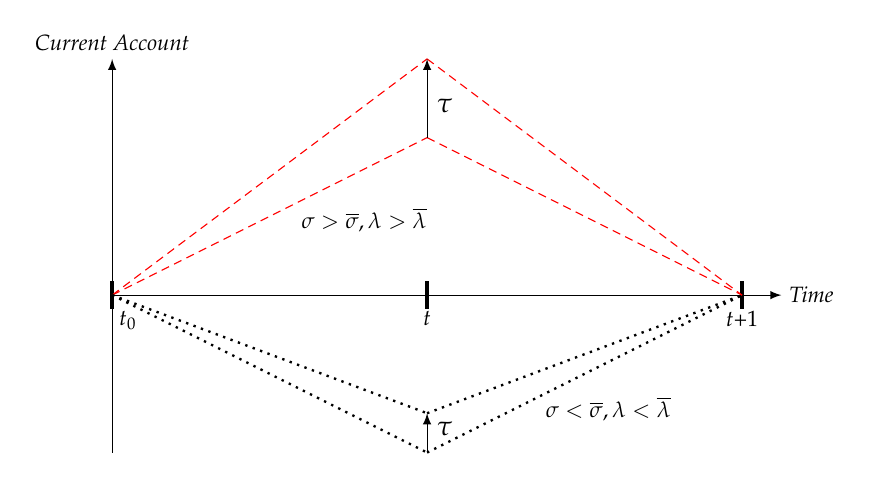
\begin{tikzpicture}[>=latex]
\draw[->] (0,0) -- (8.5,0) node[right,scale=0.8] {\textit{Time}};
      \draw[->] (0,-2) -- (0,3) node[above,scale=0.8] {\textit{Current Account}};
      \foreach \x in {0,4,8}
\draw [line width=0.5mm] (\x cm,5pt) -- (\x cm,-5pt);
\draw[] (0.2,0) node[below=3pt, scale=0.8] {$t_0$};
\draw[] (4,0) node[below=3pt, scale=0.8] {$t$};
\draw[] (8,0) node[below=3pt, scale=0.8] {$t$+$1$};
    \draw[red,densely dashed] (0,0)  -- (4,2);
    \draw[red,densely dashed] (4,2)  -- (8,0);
    \draw[red,densely dashed] (0,0)  -- (4,3);
    \draw[red,densely dashed] (4,3)  -- (8,0);
      \draw[] (4,2.4)  node[right,scale=1]{$\tau$};
            \draw[->] (4,2) -- (4,3);
    \draw[black,dotted, line width=0.3mm] (0,0)  -- (4,-2);
    \draw[black,dotted, line width=0.3mm] (4,-2)  -- (8,0);
      \draw[black,dotted, line width=0.3mm] (0,0)  -- (4,-1.5);
    \draw[black,dotted, line width=0.3mm] (4,-1.5)  -- (8,0);
    \draw[] (4,-1.7)  node[right,scale=1]{$\tau$};
            \draw[->] (4,-2) -- (4,-1.5);
        \draw[] (3.2,0.7)  node[above,scale=0.8]{$\sigma>\overline{\sigma}, \lambda>\overline{\lambda}$};
         \draw[] (6.3,-1.2)  node[below,scale=0.8]{$\sigma<\overline{\sigma}, \lambda<\overline{\lambda}$};

    \end{tikzpicture}
}

\end{subfigure}%% 
\end{center}
\footnotesize \textit{\textbf{Notes:} Panel (a): The chart illustrates that the current account is a function of volatility ($\sigma$) and investor risk aversion ($\lambda$). $\overline{\sigma}, \overline{\lambda}$ (blue line) are consistent with a zero current account. More (less) volatility or higher (lower) risk aversion implies less (more) emerging market borrowing and  a current account surplus (deficit) (dashed red and dotted black lines). 
Panel (b): The chart portrays the consequence of capital inflow controls on the current account when international financial volatility ($\sigma$) and investor risk aversion ($\lambda$) are either high (dashed red lines) or low (dotted black lines). Capital inflow controls ($\tau$) reduce borrowing; however, the tax is larger when volatility or risk aversion is high, leading to a disproportionate effect on the current account during financial turmoil.} 
\end{figure}




Capital inflow controls as specified in the previous section limit the issuance of new debt in period $t$ and thus either reduce the current account deficit when global financial conditions are calm or increase the current account surplus during periods of financial turmoil and heightened uncertainty. Figure \ref{fig:ca}, Panel (b) illustrates these observations. The dashed red lines signal a current account surplus ($\sigma>\overline{\sigma}, \lambda>\overline{\lambda}$) which increases  with the capital control tax. Similarly,  the dotted black lines indicate that the tax reduces the current account deficit during benign financial conditions. However, the effects are  disproportionate: The increase in the current account surplus exceeds the reduction in the deficit precisely because intervention increases with deteriorating financial markets, as highlighted by Propositions 1 and 2. 



Current account reversals are generally perceived as detrimental to emerging markets.  We differ from the   literature in two aspects  (see, for example, \citealp{bianchi_2011}; \citealp{korinek_2018}): First,  bonds  are more costly to issue in our model when financial conditions deteriorate. The introduction of a time-varying risk premium therefore makes  inflow restrictions during global financial distress more desirable. Second, our model abstracts from borrowing limits, which, if binding, generate undesirable current account reversals. Apart from these features we also abstract from production. If production is realistically tied to foreign investments, lowering inflows during a period of already limited access to financing could generate long-lasting adverse effects on the macroeconomy  (\citealp{ma_2020}).



\subsection{Monopoly Power Revisited} \label{sec:2eme}

The previous narrative provides a clear justification for regulatory intervention via capital inflow controls from the perspective of an emerging market, particularly during periods of international financial distress: intervention in  capital markets  reduces the  required risk premium. The incentives to reduce the cost of debt are tied to the monopoly power of the emerging market. An emerging market has a natural monopoly on its own debt -- but how relevant is this characteristic in practice? The subsequent two extensions  assess the plausibility of our analytical results. We vary the  size of the emerging market and  add a second emerging market that competes with the other emerging market for funds from international investors.


\noindent\textbf{Country Size}

Small emerging markets naturally issue less debt and are hence quantitatively less relevant in international portfolios.  As such, a regulator may have limited ability to manipulate the risk premium simply because investors are less sensitive to debt from the specific emerging market. As a consequence, our model predicts that intervention via capital controls would be muted. Indeed, this is also what we observe in the data, as Figure \ref{fig:size} emphasizes.





Concerning the model, we capture the size of an emerging market with the parameter $\chi$, which  determines the size of the country relative to the size of international investors. If $\chi$ is small, aggregate debt becomes negligible from the perspective of investors, which diminishes the responsiveness to changes in emerging market debt. Capital controls are therefore small, as we illustrate in Figure \ref{fig:size}, Panel (a).



It is reassuring that we observe a similar pattern in the data. In Panel (b) of Figure \ref{fig:size}, we provide results from a  bivariate OLS regression where we regress the  `Inflow Restriction Index' (see Section \ref{sec:emp_data}) on the size of the domestic economy as measured by GDP in USD. As apparent from the plot, the relationship between capital inflow controls and GDP, our proxy for market power, is positive and significant, particularly when we exclude outliers with a high GDP (solid blue line). 




\begin{figure}[!h] 
   \caption{Country Size and Capital Controls}
     \label{fig:size}
       \vspace{-0.5cm}
       \begin{center}
      \begin{adjustbox}{minipage=\linewidth,scale=1}
  \begin{subfigure}{0.50\linewidth}
               \caption{Model} 
    \includegraphics[width=1\linewidth]{figures/Figure_11a.pdf} 
  \end{subfigure}%% 
  \begin{subfigure}{0.50\linewidth}
               \caption{Data} 
    \includegraphics[width=1\linewidth]{figures/Figure_11b.pdf} 
  \end{subfigure} 
        \end{adjustbox}
        \end{center}
  \footnotesize \textit{\textbf{Notes}: Panel (a): The plot displays the  level of capital controls $\tau$ (y-axis) as a function of the size of the emerging market ($\chi$).  Calibration: $e_{B,t}$-$(1$+$\overline{RP})\overline{b}_{B,0}$=-$0.2$, $p$=$0.02$, $\lambda$=$1$. Panel (b): The panel presents results from a bivariate OLS regression. Dependent variable (y-axis): `Inflow Restriction Index'.  Independent variable: Domestic GDP in Billion USD. Both variables are country-specific sample averages. We add 90\% predictive margins and individual observations. GDP is trimmed (top and bottom  5\%). The regression underlying the blue line further excludes countries with a GDP of more than 550 Billion USD. Sample: 1995-2017. The panel includes both active and inactive emerging markets. See Section \ref{sec:emp_data} for more details on the data.}
\end{figure}

\noindent\textbf{Two Competing Emerging Markets}

We consider two emerging markets (`domestic' and `foreign') that compete for funds from international investors. We model both emerging markets equivalently, that is, both emerging markets follow the same setup as described in Section \ref{sec:environment}.  We denote the default probability of the second (foreign) emerging market as $q(\sigma)$ with $\frac{\partial q(\sigma)}{\partial \sigma}>0$. The most notable difference between the basic setup and this extended framework pertains to the default structure among both emerging markets. To be more precise, we define the probability that \textit{both} emerging markets default on their debt as $d$, where $d$ is necessarily smaller than $p$ or $q$, that is, $d\leq min\{p,q\}$. Consequently,  we can determine four regimes. We display these regimes and their associated probabilities in Figure \ref{fig:corr_structure}.



\begin{figure}[h]
\begin{center}
\caption{Payoff Structure}
 \label{fig:corr_structure} 
\scalebox{1.00}{
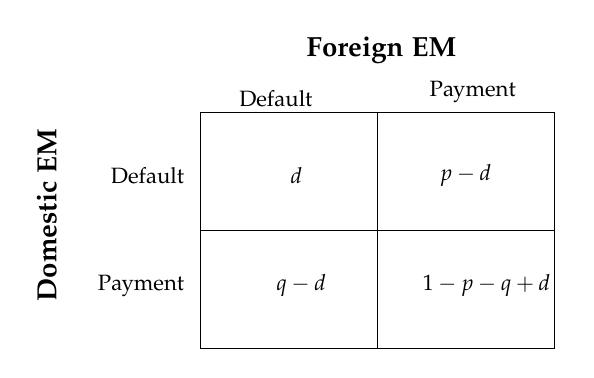
\begin{tikzpicture}[>=latex]
\node[align=center,  above] at (2.8,2.5) {\textbf{Foreign EM}};
\node[align=center, font=\footnotesize,  above] at (1.5,1.95) {Default };
\node[align=center, font=\footnotesize,  above] at (4,2) {Payment };
\node[align=center, font=\footnotesize,  left] at (0.5,1.2) {Default };
\node[align=center, font=\footnotesize,  left] at (2.0,1.2) {$d$ };
\node[align=center, font=\footnotesize,  left] at (4.4,1.2) {$p-d$ };
\node[align=center, font=\footnotesize,  left] at (0.5,-0.2) {Payment };
\node[align=center, font=\footnotesize,  left] at (2.3,-0.2) {$q-d$ };
\node[align=center, font=\footnotesize,  left] at (5.15,-0.2) {$1-p-q+d$ };
\draw[draw=black] (5,2) rectangle (0.5,-1);
\draw (5,0.5) -- (0.5,0.5);
\draw (2.75,2) -- (2.75,-1);
\node[align=center,  above, rotate=90] at (-1.2,0.7) {\textbf{Domestic EM}};


\end{tikzpicture}
}
 \end{center}
 \end{figure}
 
 
 In this extended framework, international investors  can choose between three assets, the riskless asset and two risky emerging market bonds. Their optimization problem is therefore summarized as:
 
 \begin{equation}  \tag{Po:I}
   \max_{c_{I,t+1},  b_{I,t+1}, b_{I,t+1}^*  l_{t+1}} \big\{ E_t[v_{t+1}(c_{I,t+1})]\big\},
\end{equation}

\noindent where we characterize foreign variables with an asterisk ($^*$).  The augmented budget constraints  are: 


\begin{align}
b_{I,t+1}+b_{I,t+1}^*+l_{t+1} &=e_{I,t}+(1+\overline{RP})\overline{b}_{I,0}+(1+\overline{RP}^*)\overline{b}^*_{I,0} \label{eq:2em_1} \\
\overline{b}_{I,T}+\overline{b}^*_{I,T}+c_{I,t+1} &= (1+RP_t) \tilde{b}_{I,t+1}+(1+RP_t^*) \tilde{b}_{I,t+1}^*+ l_{t+1} +a_{t+1}. \label{eq:2em_2}
\end{align}

\noindent We analyze capital controls in a Nash equilibrium where both emerging markets resort to capital controls in a non-cooperative manner.\footnote{Emerging markets tend to impose capital controls unilaterally. If both emerging markets in our setup cooperate, they would be able to levy a larger tax and extract more rent from international investors in line with Figure \ref{fig:size}, Panel (a).}  Figure \ref{fig:tax_d} portrays the  level of capital controls as a function of the probability that both emerging markets default ($d$). Because  default is  Bernoulli distributed, $d$ also captures the correlation in the risk profile among both emerging markets.  Specifically, if $d>pq$, default among the two emerging markets is positively correlated. On an abstract level, we can interpret $d$ as the co-movement of business cycles given that default is more likely during recessions. Based on the chart, it becomes apparent that capital inflow restrictions increase with a more similar risk structure. Intuitively, if  default probabilities are negatively correlated, investors can purchase both bonds in equal amounts (complements) and thus mitigate the aggregate risk from emerging market bonds.  Consequently, the aggregate demand curve flattens, and the wedge between the regulated and the unregulated equilibrium declines. In reality, many emerging markets face similar business cycle dynamics, especially countries that are geographically close. Hence, the fact that countries compete for funds does not necessarily imply that countries should impose fewer capital controls, even when the sole motivation for capital controls relates to monopolistic interventions to reduce the debt burden and risk premium.




\begin{figure}[!h] 
  \begin{center}
  	 \caption{Two Emerging Markets: The Correlation Structure and Capital Controls}
    \includegraphics[width=0.55\linewidth]{figures/Figure_13.pdf}      \label{fig:tax_d}
  \end{center}
       \vspace{-0.3cm}
  \footnotesize \textit{\textbf{Notes}: The plot displays the  level of capital inflow controls $\tau$ (y-axis) as a function of the probability that both emerging markets default simultaneously.    Calibration: $\chi$=$1$, $e_{B,t}$-$(1$+$\overline{RP})\overline{b}_{B,0}$=-$0.2$, $p$=$q$=$0.02$, $\lambda$=$1$. Both countries are identical.} 
\end{figure}





\section{Conclusion}

Capital controls receive significant attention from international policymakers as a tool to mitigate boom-bust cycles in international financial flows and to limit external overborrowing. However, though emerging markets make heavy use of capital controls, it is not well understood why they are used in practice. For example, while the theoretical literature advocates macroprudential capital inflow controls when an economy is at risk and subject to substantial capital inflows, the applied literature has not been able to observe such patterns except for a few case studies. A natural question is why countries have not implemented capital controls accordingly. 

 In this paper, we emphasize an alternative rationale to impose capital controls. We first document a new stylized fact: countries that actively reevaluate their capital inflow controls respond to deteriorating global financial conditions -- in particular elevated volatility and risk aversion -- by tightening capital inflow restrictions.  We then  propose a simple model that rationalizes the empirical finding. In the model, regulators have an incentive to tax capital inflows to lower borrowing costs. This desire is particularly strong when investors are very sensitive to emerging market risk and demand a high premium as during global financial crises. 
 
 Our results come with two caveats: First,  while we justify capital inflow controls during periods of heightened international financial distress, this intervention is only optimal from the perspective of the emerging market at the expense of international investors.   Second, after the Global Financial Crisis, there has been a steady trend towards macroprudential capital controls, likely due to the updated IMF view and recent theoretical advances. As such, the positive relationship between financial turmoil and capital inflow controls may  fade in the future.




\clearpage 	

\appendix
\clearpage



\setcounter{table}{0}						
\renewcommand{\thetable}{A\arabic{table}}
	
\setcounter{figure}{0}					
\renewcommand{\thefigure}{A\arabic{figure}}	

%%%%%%%%%%%%%%%%%%%%%%%%%%%%%%%%%%%%%%%%%%%%%%%%%%%%%


\section{Appendix: Tables}\label{sec:appendix_tables}



\begin{table}[!htb]
\begin{center}
  \caption{Country List - Active and Inactive} 
  \label{tab:countries} 
\scalebox{\tablescale}{
\begin{tabular}{@{\extracolsep{5pt}}llll}
\toprule 
Algeria & Egypt & Mexico & South Africa \\
Angola & El Salvador & Moldova & Sri Lanka \\
Argentina & Ethiopia & Morocco & Swaziland \\
Bahrain & Georgia & Myanmar & Tanzania \\
Bangladesh & Ghana & Nicaragua & Thailand \\
Bolivia & Guatemala & Nigeria & Togo \\
Brazil & Hungary & Oman & Tunisia \\
Brunei Darussalam & India & Pakistan & Turkey \\
Bulgaria & Indonesia & Panama & Uganda \\
Burkina Faso & Jamaica & Paraguay & Ukraine \\
Chile & Kazakhstan & Peru & United Arab Emirates \\
China & Kenya & Philippines & Uruguay \\
Colombia & Kuwait & Poland & Uzbekistan \\
Costa Rica & Kyrgyz Republic & Qatar & Venezuela \\
Côte d'Ivoire & Lebanon & Romania & Vietnam \\
Dominican Republic & Malaysia & Russia & Yemen \\
 Ecuador & Mauritius & Saudi Arabia & Zambia \\ 
 \bottomrule
\end{tabular}
  }
\end{center}
\end{table}

\begin{table}[!h]
\begin{center}
\def\sym#1{\ifmmode^{#1}\else\(^{#1}\)\fi}
\caption{Default in Emerging Markets and Financial Distress}
\label{tab:calibration_p}
\scalebox{\tablescale}{
\begin{tabular}{l*{6}{c}}
\toprule
                &\multicolumn{6}{c}{External Debt Crisis}  \\
                &\multicolumn{3}{c}{Active Countries} &\multicolumn{3}{c}{All Countries}   \\
                &\multicolumn{1}{c}{(1)}   &\multicolumn{1}{c}{(2)}   &\multicolumn{1}{c}{(3)}   &\multicolumn{1}{c}{(4)} 
                &\multicolumn{1}{c}{(5)}   &\multicolumn{1}{c}{(6)}  \\ 
\midrule
$ ln(VIX) $     &     0.12   &            &            &     0.24   &            &            \\
                &   (0.41)   &            &            &   (0.27)   &            &            \\
[1em]
$ ln(VIX)_{-1} $&            &     0.35*  &            &            &     0.44***&            \\
                &            &   (0.19)   &            &            &   (0.16)   &            \\
[1em]
$ ln(VOL)_{-1} $&            &            &     0.29*  &            &            &     0.35***\\
                &            &            &   (0.15)   &            &            &   (0.14)   \\
\midrule
Pseudo $ R^2 $  &    0.002   &    0.012   &    0.009   &    0.005   &    0.017   &    0.013   \\
Observations    &      208   &      195   &      195   &      672   &      630   &      630   \\
\bottomrule
\end{tabular}
}
\end{center}
\footnotesize \textit{\textbf{Notes}: The table presents results from  bivariate logit models. Dependent variable: Start of external debt crisis (\citealp{reinhart_2009}).  ln(VIX) and ln(VOL) are standardized. We estimate a constant, but do not display it here.  Sample: 1995-2010. Huber-White robust standard errors are in parentheses. Stars indicate significance levels (*10\%, **5\%, ***1\%).}
\end{table}


\begin{table}[!h]
\begin{center}
\caption{Active versus Inactive Countries}
\label{tab:descstat} 
\scalebox{\tablescale}{
\begin{tabular}{lcc} \toprule
 & Active  & Inactive \\  \midrule
Inflow Restriction Index  &      0.483 &        0.423 \\   
  CA/GDP (in \%)  &      -2.2166 &       -0.342 \\  
 Credit/GDP (in \%) &        34.024 &       44.618 \\   
 Inst. Quality &         63.146 &       63.724 \\   
 GDP, Billions USD  &    251.775 &      217.588 \\  
Exchange Rate (CV) &          0.572 &        0.355 \\ 
Banking Crisis (in \%) &       2.372 &        1.796 \\  
\bottomrule
\end{tabular}
}
\end{center}
\footnotesize \textit{\textbf{Notes}: Comparison between emerging markets which actively adjust their capital inflow restrictions and the remaining (inactive) countries.  Institutional Quality is the sum over 12 different  categories. The highest score for each category is 12.  The exchange rate statistic displays the coefficient of variation (standard deviation/mean). All variables are sample averages. Sample: 1995-2017.}
\end{table}




\begin{table}[!h]
\begin{center}
\def\sym#1{\ifmmode^{#1}\else\(^{#1}\)\fi}
\caption{Comparison: VIX, Risk Aversion and Volatility} \label{tab:components}
\scalebox{\tablescale}{
\begin{tabular}{l*{6}{p{1.5cm}}}
\toprule
                 &\multicolumn{3}{c}{Increase in Inflow Restrictions}   & \multicolumn{3}{c}{        Decrease in Inflow Restrictions}  \\
                &\multicolumn{1}{c}{(1)}   &\multicolumn{1}{c}{(2)}   &\multicolumn{1}{c}{(3)}   &\multicolumn{1}{c}{(4)}   &\multicolumn{1}{c}{(5)}   &\multicolumn{1}{c}{(6)}   \\
\midrule
$ ln(VIX) $     &     0.36   &            &            &   -53.58   &            &            \\
                &  (32.04)   &            &            &  (34.24)   &            &            \\
\addlinespace
$ ln(VIX) $ $\times$ $ ln(VIX) $&    -0.12   &            &            &     6.04   &            &            \\
                &   (3.41)   &            &            &   (3.68)   &            &            \\
\addlinespace
$ ln(VIX) $ $\times$ $ ln(VIX) $ $\times$ $ ln(VIX) $&     0.01   &            &            &    -0.22*  &            &            \\
                &   (0.12)   &            &            &   (0.13)   &            &            \\
\addlinespace
$ ln(RA) $      &            &    -7.56   &            &            &   -32.26** &            \\
                &            &  (14.79)   &            &            &  (15.34)   &            \\
\addlinespace
$ ln(RA) $ $\times$ $ ln(RA) $&            &     1.23   &            &            &     5.88** &            \\
                &            &   (2.57)   &            &            &   (2.70)   &            \\
\addlinespace
$ ln(RA) $ $\times$ $ ln(RA) $ $\times$ $ ln(RA) $&            &    -0.06   &            &            &    -0.35** &            \\
                &            &   (0.15)   &            &            &   (0.16)   &            \\
\addlinespace
$ ln(VOL) $     &            &            &    16.55   &            &            &    -4.97   \\
                &            &            &  (30.71)   &            &            &  (35.18)   \\
\addlinespace
$ ln(VOL) $ $\times$ $ ln(VOL) $&            &            &    -1.60   &            &            &     0.72   \\
                &            &            &   (2.91)   &            &            &   (3.38)   \\
\addlinespace
$ ln(VOL) $ $\times$ $ ln(VOL) $ $\times$ $ ln(VOL) $&            &            &     0.05   &            &            &    -0.03   \\
                &            &            &   (0.09)   &            &            &   (0.11)   \\
\midrule
p-value: VIX RA/VOL $=0 $&    0.026   &    0.052   &    0.023   &    0.074   &    0.051   &    0.350   \\
Pseudo $ R^2 $  &    0.019   &    0.017   &    0.020   &    0.016   &    0.015   &    0.009   \\
Observations    &      483   &      483   &      483   &      483   &      483   &      483   \\
\bottomrule
\end{tabular}
}
\end{center}
\footnotesize \textit{\textbf{Notes}:   ln(VIX), ln(RA) and ln(VOL) are standardized. We estimate a constant, but do not display it here. The p-value at the bottom of the table is based on a hypothesis test examining whether all VIX/RA/VOL related coefficients are jointly zero.  Calculations based on active emerging markets only. Sample: 1995-2017. Huber-White robust standard errors are in parentheses. Stars indicate significance levels (*10\%, **5\%, ***1\%).} 
\end{table}

\begin{table}[h!]
 \begin{center}
\def\sym#1{\ifmmode^{#1}\else\(^{#1}\)\fi}
\caption{Robustness: Control Variables} \label{tab:logit}
\scalebox{\tablescale}{
\begin{tabular}{l*{6}{c}}
\toprule
                    &\multicolumn{3}{c}{Increase in Inflow Restrictions}                   &\multicolumn{3}{c}{Decrease in Inflow Restrictions}                           \\
                    &\multicolumn{1}{c}{(1)}   &\multicolumn{1}{c}{(2)}   &\multicolumn{1}{c}{(3)}   &\multicolumn{1}{c}{(4)}
                    &\multicolumn{1}{c}{(5)}
                    &\multicolumn{1}{c}{(6)}\\
\midrule
$ ln(VIX) $         &        0.39***&       14.19   &        8.56   &        0.10   &      -67.28*  &      -63.91*  \\
                    &      (0.14)   &     (33.48)   &     (34.18)   &      (0.12)   &     (35.71)   &     (36.48)   \\
\addlinespace
$ ln(VIX) $ $\times$ $ ln(VIX) $&               &       -1.61   &       -0.99   &               &        7.46*  &        7.09*  \\
                    &               &      (3.57)   &      (3.65)   &               &      (3.83)   &      (3.93)   \\
\addlinespace
$ ln(VIX) $ $\times$ $ ln(VIX) $ $\times$ $ ln(VIX) $&               &        0.06   &        0.04   &               &       -0.27** &       -0.26*  \\
                    &               &      (0.13)   &      (0.13)   &               &      (0.14)   &      (0.14)   \\
\addlinespace
$ \Delta CA/GDP_{-1} $&               &               &       -0.02   &               &               &       -0.03   \\
                    &               &               &      (0.03)   &               &               &      (0.03)   \\
\addlinespace
$ \Delta log(GDP)_{-1} $&               &               &        0.03   &               &               &       -0.04   \\
                    &               &               &      (0.04)   &               &               &      (0.04)   \\
\addlinespace
$ \Delta log(Exchange Rate)_{-1} $&               &               &        0.00   &               &               &        0.00   \\
                    &               &               &      (0.01)   &               &               &      (0.01)   \\
\addlinespace
$ Inst. Quality_{-1} $&               &               &       -0.06   &               &               &        0.17   \\
                    &               &               &      (0.12)   &               &               &      (0.12)   \\
\addlinespace
$ Banking Crisis_{-1} $&               &               &       -0.20   &               &               &        0.28   \\
                    &               &               &      (0.82)   &               &               &      (0.76)   \\
\midrule
p-value: VIX $=0$      &       0.005   &       0.014   &       0.027   &       0.374   &       0.066   &       0.144   \\
Pseudo $ R^2 $      &       0.022   &       0.025   &       0.028   &       0.002   &       0.018   &       0.027   \\
Observations        &     427  &     427  &     427   &     427   &     427  &     427  \\
\bottomrule

\end{tabular}
}
\end{center}
\footnotesize \textit{\textbf{Notes}: Institutional quality and ln(VIX) are standardized. Banking crisis is a binary indicator equal to one if a crisis occurs. The remaining variables are expressed in \%. All 'domestic' variables are lagged by one period to mitigate reverse causality concerns. We estimate a constant, but do not display it here. The p-value at the bottom of the table is based on a hypothesis test examining whether all VIX related coefficients are jointly zero.  Calculations based on active emerging markets only. Sample: 1995-2017. Huber-White robust standard errors are in parentheses. Stars indicate significance levels (*10\%, **5\%, ***1\%).} 
\end{table}





\begin{table}[!h]
\begin{center}
\def\sym#1{\ifmmode^{#1}\else\(^{#1}\)\fi}
\caption{Additional Domestic Variables: Increase in Inflow Restrictions}
\label{tab:add-dom-vars-i}
\scalebox{\tablescale}{
\begin{tabular}{l*{4}{p{1cm}}}
\toprule
                &\multicolumn{4}{c}{Increase in Inflow Restrictions}     \\
                &\multicolumn{1}{c}{(1)}   &\multicolumn{1}{c}{(2)}   &\multicolumn{1}{c}{(3)}     &\multicolumn{1}{c}{(4)}    \\
\midrule
$ ln(VIX) $     &     8.56   &    21.43   &    13.85   &     6.50   \\
                &  (34.18)   &  (42.87)   &  (38.65)   &  (35.88)   \\
\addlinespace
$ ln(VIX) $ $\times$ $ ln(VIX) $&    -0.99   &    -2.26   &    -1.48   &    -0.77   \\
                &   (3.65)   &   (4.61)   &   (4.12)   &   (3.84)   \\
\addlinespace
$ ln(VIX) $ $\times$ $ ln(VIX) $ $\times$ $ ln(VIX) $&     0.04   &     0.08   &     0.05   &     0.03   \\
                &   (0.13)   &   (0.16)   &   (0.15)   &   (0.14)   \\
\addlinespace
$ \Delta CA/GDP_{-1} $&    -0.02   &    -0.06   &    -0.01   &    -0.02   \\
                &   (0.03)   &   (0.05)   &   (0.04)   &   (0.03)   \\
\addlinespace
$ \Delta log(GDP)_{-1} $&     0.03   &     0.02   &     0.02   &     0.07*  \\
                &   (0.04)   &   (0.05)   &   (0.04)   &   (0.04)   \\
\addlinespace
$ \Delta log(Exchange Rate)_{-1} $&     0.00   &    -0.00   &     0.01   &     0.01   \\
                &   (0.01)   &   (0.01)   &   (0.01)   &   (0.01)   \\
\addlinespace
$ Inst. Quality_{-1} $&    -0.06   &    -0.01   &    -0.16   &     0.10   \\
                &   (0.12)   &   (0.15)   &   (0.13)   &   (0.33)   \\
\addlinespace
$ Banking Crisis_{-1} $&    -0.20   &     0.69   &    -1.04   &    -0.35   \\
                &   (0.82)   &   (1.40)   &   (0.90)   &   (0.95)   \\
\addlinespace
$ \Delta log(Stock Index)_{-1} $&            &     0.01** &            &            \\
                &            &   (0.01)   &            &            \\
\addlinespace
$ \Delta (Credit/GDP)_{-1} $&            &            &     0.03   &            \\
                &            &            &   (0.03)   &            \\
\midrule
Fixed Effects &    No   &    No  &      No   &       Yes   \\
p-value: VIX $=0$  &    0.027   &    0.105   &    0.029   &    0.034   \\
Pseudo $ R^2 $  &    0.028   &    0.066   &    0.040   &    0.113    \\
Observations    &  427   &  271   &  354   &  427   \\
\bottomrule
\end{tabular}
}
\end{center}
\footnotesize \textit{\textbf{Notes}: Institutional quality and ln(VIX) are standardized. Banking crisis is a binary indicator equal to one if a crisis occurs. The remaining variables are expressed in \%. All 'domestic' variables are lagged by one period to mitigate reverse causality concerns. We estimate a constant, but do not display it here.  The p-value at the bottom of the table is based on a hypothesis test examining whether all VIX related coefficients are jointly zero.  Calculations based on active emerging markets only.   Sample: 1995-2017. Huber-White robust standard errors are in parentheses. Stars indicate significance levels (*10\%, **5\%, ***1\%).} 
\end{table}

\begin{table}[!h]
\begin{center}
\def\sym#1{\ifmmode^{#1}\else\(^{#1}\)\fi}
\caption{Additional Domestic Variables: Decrease in Inflow Restrictions}
\label{tab:add-dom-vars-d}
\scalebox{\tablescale}{
\begin{tabular}{l*{4}{p{1cm}}}
\toprule
                &\multicolumn{4}{c}{Decrease in Inflow Restrictions}     \\
&\multicolumn{1}{c}{(1)}   &\multicolumn{1}{c}{(2)}   &\multicolumn{1}{c}{(3)}     &\multicolumn{1}{c}{(4)}        \\
\midrule
$ ln(VIX) $     &   -63.91*  &   -66.43   &   -78.38** &   -62.80*  \\
                &  (36.48)   &  (43.29)   &  (39.23)   &  (36.87)   \\
\addlinespace
$ ln(VIX) $ $\times$ $ ln(VIX) $&     7.09*  &     7.12   &     8.56** &     6.98*  \\
                &   (3.93)   &   (4.67)   &   (4.24)   &   (3.96)   \\
\addlinespace
$ ln(VIX) $ $\times$ $ ln(VIX) $ $\times$ $ ln(VIX) $&    -0.26*  &    -0.25   &    -0.31** &    -0.26*  \\
                &   (0.14)   &   (0.17)   &   (0.15)   &   (0.14)   \\
\addlinespace
$ \Delta CA/GDP_{-1} $&    -0.03   &    -0.07   &    -0.04   &    -0.03   \\
                &   (0.03)   &   (0.05)   &   (0.04)   &   (0.03)   \\
\addlinespace
$ \Delta log(GDP)_{-1} $&    -0.04   &    -0.06   &    -0.04   &    -0.06   \\
                &   (0.04)   &   (0.05)   &   (0.04)   &   (0.04)   \\
\addlinespace
$ \Delta log(Exchange Rate)_{-1} $&     0.00   &     0.01   &    -0.01   &    -0.00   \\
                &   (0.01)   &   (0.01)   &   (0.01)   &   (0.01)   \\
\addlinespace
$ Inst. Quality_{-1} $&     0.17   &     0.27*  &     0.15   &     0.25   \\
                &   (0.12)   &   (0.16)   &   (0.13)   &   (0.32)   \\
\addlinespace
$ Banking Crisis_{-1} $&     0.28   &     0.62   &     0.86   &     0.22   \\
                &   (0.76)   &   (1.34)   &   (0.79)   &   (0.83)   \\
\addlinespace
$ \Delta log(Stock Index)_{-1} $&            &     0.01** &            &            \\
                &            &   (0.01)   &            &            \\
\addlinespace
$ \Delta (Credit/GDP)_{-1} $&            &            &    -0.03   &            \\
                &            &            &   (0.03)   &            \\
\midrule
Fixed Effects &    No   &    No  &      No   &       Yes   \\
p-value: VIX $=0$  &    0.144   &    0.454   &    0.221   &    0.148   \\
Pseudo $ R^2 $  &    0.027   &    0.048   &    0.031   &    0.082   \\
Observations    &  427   &  271  &  354   &  427  \\
\bottomrule
\end{tabular}
}
\end{center}
\footnotesize \textit{\textbf{Notes}: Institutional quality and ln(VIX) are standardized. Banking crisis is a binary indicator equal to one if a crisis occurs. The remaining variables are expressed in \%. All 'domestic' variables are lagged by one period to mitigate reverse causality concerns.  We estimate a constant, but do not display it here.  The p-value at the bottom of the table is based on a hypothesis test examining whether all VIX related coefficients are jointly zero. Calculations based on active emerging markets only.  Sample: 1995-2017. Huber-White robust standard errors are in parentheses. Stars indicate significance levels (*10\%, **5\%, ***1\%).} 
\end{table}



\begin{table}[!h]
\begin{center}
\def\sym#1{\ifmmode^{#1}\else\(^{#1}\)\fi}
\caption{Robustness: Lenient Threshold Classification} \label{tab:80th}
\scalebox{\tablescale}{
\begin{tabular}{l*{6}{c}}
\toprule
                &\multicolumn{3}{c}{Increase in Inflow Restrictions}   & \multicolumn{3}{c}{           Decrease in Inflow Restrictions}             \\
                &\multicolumn{1}{c}{(1)}   &\multicolumn{1}{c}{(2)}   &\multicolumn{1}{c}{(3)}   &\multicolumn{1}{c}{(4)}   &\multicolumn{1}{c}{(5)}   &\multicolumn{1}{c}{(6)}   \\
\midrule
$ ln(VIX) $         &        0.24** &       -0.51   &       -0.27   &        0.11   &      -55.90*  &      -54.16*  \\
                    &      (0.12)   &     (30.04)   &     (30.77)   &      (0.10)   &     (31.91)   &     (32.62)   \\
\addlinespace
$ ln(VIX) $ $\times$ $ ln(VIX) $&               &       -0.06   &       -0.09   &               &        6.31*  &        6.11*  \\
                    &               &      (3.20)   &      (3.28)   &               &      (3.42)   &      (3.50)   \\
\addlinespace
$ ln(VIX) $ $\times$ $ ln(VIX) $ $\times$ $ ln(VIX) $&               &        0.01   &        0.01   &               &       -0.23*  &       -0.23*  \\
                    &               &      (0.11)   &      (0.12)   &               &      (0.12)   &      (0.12)   \\
\addlinespace
$ \Delta CA/GDP_{-1} $&               &               &       -0.02   &               &               &       -0.03   \\
                    &               &               &      (0.03)   &               &               &      (0.03)   \\
\addlinespace
$ \Delta log(GDP)_{-1} $&               &               &       -0.01   &               &               &        0.01   \\
                    &               &               &      (0.03)   &               &               &      (0.03)   \\
\addlinespace
$ \Delta log(Exchange Rate)_{-1} $&               &               &        0.00   &               &               &        0.01   \\
                    &               &               &      (0.01)   &               &               &      (0.01)   \\
\addlinespace
$ Inst. Quality_{-1} $&               &               &        0.00   &               &               &        0.14   \\
                    &               &               &      (0.11)   &               &               &      (0.12)   \\
\addlinespace
$ Banking Crisis_{-1} $&               &               &        0.13   &               &               &        0.09   \\
                    &               &               &      (0.61)   &               &               &      (0.63)   \\
\midrule
p-value: VIX $=0$      &       0.041   &       0.101   &       0.144   &       0.272   &       0.020   &       0.051   \\
Pseudo $ R^2 $      &       0.008   &       0.011   &       0.012   &       0.002   &       0.019   &       0.025   \\
Observations    &      556   &      556   &      556   &      556   &      556   &      556   \\
\bottomrule
\end{tabular}
}
\end{center}
\footnotesize \textit{\textbf{Notes}: This table provides result from a more lenient classification requirement (domestic std. dev. above 0.8 of avg. std. dev.). This lower threshold classifies six more countries as active: Bolivia (std. dev. 0.101), Saudi Arabia (0.100), Romania (0.95), Ukraine (0.094), Dominican Republic (0.89) and Jamaica (0.85). Institutional quality and ln(VIX) are standardized. Banking crisis is a binary indicator equal to one if a crisis occurs. The remaining variables are expressed in \%. All 'domestic' variables are lagged by one period to mitigate reverse causality concerns. We estimate a constant, but do not display it here. The p-value at the bottom of the table is based on a hypothesis test examining whether all VIX related coefficients are jointly zero. 
 Calculations based on active emerging markets only. Sample: 1995-2017. Huber-White robust standard errors are in parentheses. Stars indicate significance levels (*10\%, **5\%, ***1\%).} 
\end{table}

\begin{table}[!h]
\begin{center}
\def\sym#1{\ifmmode^{#1}\else\(^{#1}\)\fi}
\caption{Robustness: Strict Threshold Classification} \label{tab:120th}
\scalebox{\tablescale}{
\begin{tabular}{l*{6}{c}}
\toprule
                &\multicolumn{3}{c}{Increase in Inflow Restrictions}   & \multicolumn{3}{c}{           Decrease in Inflow Restrictions}             \\
                &\multicolumn{1}{c}{(1)}   &\multicolumn{1}{c}{(2)}   &\multicolumn{1}{c}{(3)}   &\multicolumn{1}{c}{(4)}   &\multicolumn{1}{c}{(5)}   &\multicolumn{1}{c}{(6)}   \\
\midrule
$ ln(VIX) $         &        0.48***&       15.21   &        7.83   &        0.07   &      -94.89** &      -94.06** \\
                    &      (0.18)   &     (41.07)   &     (43.66)   &      (0.14)   &     (44.14)   &     (45.41)   \\
\addlinespace
$ ln(VIX) $ $\times$ $ ln(VIX) $&               &       -1.83   &       -1.01   &               &       10.43** &       10.33** \\
                    &               &      (4.38)   &      (4.65)   &               &      (4.76)   &      (4.91)   \\
\addlinespace
$ ln(VIX) $ $\times$ $ ln(VIX) $ $\times$ $ ln(VIX) $&               &        0.07   &        0.04   &               &       -0.38** &       -0.38** \\
                    &               &      (0.15)   &      (0.16)   &               &      (0.17)   &      (0.18)   \\
\addlinespace
$ \Delta CA/GDP_{-1} $&               &               &       -0.01   &               &               &       -0.06   \\
                    &               &               &      (0.04)   &               &               &      (0.04)   \\
\addlinespace
$ \Delta log(GDP)_{-1} $&               &               &        0.07*  &               &               &       -0.04   \\
                    &               &               &      (0.04)   &               &               &      (0.04)   \\
\addlinespace
$ \Delta log(Exchange Rate)_{-1} $&               &               &        0.01   &               &               &       -0.00   \\
                    &               &               &      (0.01)   &               &               &      (0.01)   \\
\addlinespace
$ Inst. Quality_{-1} $&               &               &       -0.10   &               &               &        0.14   \\
                    &               &               &      (0.13)   &               &               &      (0.14)   \\
\addlinespace
$ Banking Crisis_{-1} $&               &               &       -0.72   &               &               &       -0.64   \\
                    &               &               &      (1.12)   &               &               &      (1.13)   \\
\midrule
p-value: VIX $=0$      &       0.007   &       0.007   &       0.008   &       0.644   &       0.097   &       0.159   \\
Pseudo $ R^2 $      &       0.032   &       0.042   &       0.058   &       0.001   &       0.026   &       0.040   \\
Observations    &      281   &      281   &      281   &      281   &      281   &      281   \\
\bottomrule

\end{tabular}
}
\end{center}
\footnotesize \textit{\textbf{Notes}: This table provides result from a more strict classification requirement (domestic std. dev. above 1.2 of avg. std. dev.). With this tighter threshold only 14 countries are classified as active with Vietnam as the last country included (see Table \ref{tab:active_countries}). Institutional quality and ln(VIX) are standardized. Banking crisis is a binary indicator equal to one if a crisis occurs. The remaining variables are expressed in \%. All 'domestic' variables are lagged by one period to mitigate reverse causality concerns. We estimate a constant, but do not display it here. The p-value at the bottom of the table is based on a hypothesis test examining whether all VIX related coefficients are jointly zero.  Calculations based on active emerging markets only. Sample: 1995-2017. Huber-White robust standard errors are in parentheses. Stars indicate significance levels (*10\%, **5\%, ***1\%).} 
\end{table}






\begin{table}[!h]
\begin{center}
\def\sym#1{\ifmmode^{#1}\else\(^{#1}\)\fi}
\caption{Robustness: Chinn-Ito Index } \label{tab:chinn-ito1}
\scalebox{\tablescale}{
\begin{tabular}{l*{6}{c}}
\toprule
                &\multicolumn{3}{c}{Increase in  Restrictions}   &  \multicolumn{3}{c}{ Decrease in  Restrictions}            \\
                &\multicolumn{1}{c}{(1)}   &\multicolumn{1}{c}{(2)}   &\multicolumn{1}{c}{(3)}   &\multicolumn{1}{c}{(4)}   &\multicolumn{1}{c}{(5)}   &\multicolumn{1}{c}{(6)}   \\
\midrule
$ ln(VIX) $     &     0.34*  &    18.52   &    29.72   &     0.26   &   -52.58   &   -52.63   \\
                &   (0.19)   &  (68.44)   &  (69.99)   &   (0.16)   &  (41.77)   &  (42.94)   \\
\addlinespace
$ ln(VIX) $ $\times$ $ ln(VIX) $&            &    -1.92   &    -3.26   &            &     6.23   &     6.24   \\
                &            &   (7.72)   &   (7.92)   &            &   (4.83)   &   (4.97)   \\
\addlinespace
$ ln(VIX) $ $\times$ $ ln(VIX) $ $\times$ $ ln(VIX) $&            &     0.07   &     0.12   &            &    -0.24   &    -0.24   \\
                &            &   (0.29)   &   (0.30)   &            &   (0.18)   &   (0.19)   \\
\addlinespace
$ \Delta CA/GDP_{-1} $&            &            &    -0.03   &            &            &     0.01   \\
                &            &            &   (0.05)   &            &            &   (0.04)   \\
\addlinespace
$ \Delta log(GDP)_{-1} $&            &            &    -0.05   &            &            &     0.01   \\
                &            &            &   (0.05)   &            &            &   (0.04)   \\
\addlinespace
$ \Delta log(Exchange Rate)_{-1} $&            &            &     0.00   &            &            &    -0.00   \\
                &            &            &   (0.01)   &            &            &   (0.01)   \\
\addlinespace
$ Inst. Quality_{-1} $&            &            &     0.25   &            &            &     0.19   \\
                &            &            &   (0.18)   &            &            &   (0.17)   \\
\addlinespace
$ Banking Crisis_{-1} $&            &            &     0.57   &            &            &    -0.51   \\
                &            &            &   (0.81)   &            &            &   (1.09)   \\
\midrule
p-value: VIX $=0 $&    0.069   &    0.401   &    0.584   &    0.110   &    0.256   &    0.321   \\
Pseudo $ R^2 $  &    0.012   &    0.014   &    0.030   &    0.008   &    0.014   &    0.021   \\
Observations    &      426   &      426   &      426   &      426   &      426   &      426   \\
\bottomrule
\end{tabular}
}
\end{center}
\footnotesize \textit{\textbf{Notes}: We classify countries into active and inactive using our baseline metric, but use the Chinn-Ito Index to construct the `Increase' and `Decrease' indicators. Institutional quality and ln(VIX) are standardized. Banking crisis is a binary indicator equal to one if a crisis occurs. The remaining variables are expressed in \%. All 'domestic' variables are lagged by one period to mitigate reverse causality concerns. We estimate a constant, but do not display it here. The p-value at the bottom of the table is based on a hypothesis test examining whether all VIX related coefficients are jointly zero.  Calculations based on active emerging markets only. Sample: 1995-2017. Huber-White robust standard errors are in parentheses. Stars indicate significance levels (*10\%, **5\%, ***1\%).} 
\end{table}




\clearpage

\setcounter{table}{0}						
\renewcommand{\thetable}{B\arabic{table}}
	
\setcounter{figure}{0}					
\renewcommand{\thefigure}{B\arabic{figure}}	

%%%%%%%%%%%%%%%%%%%%%%%%%%%%%%%%%%%%%%%%%%%%%%%%%%%%%

\section{Appendix: Figures}\label{sec:appendix_figures}





 \begin{figure}[!h] 
  \caption{External Debt Crises: Emerging Markets}
     \label{fig:debt_crises}
     \vspace{-0.5cm}
  \begin{center}
    \includegraphics[width=0.60\linewidth]{figures/Figure_B1.pdf} 
  \end{center}
  \footnotesize \textit{\textbf{Notes}: The graph depicts the share of emerging markets in an ongoing external debt crisis as defined in \citet{reinhart_2009} between 1995 and 2010 in \%. We include all active and passive emerging markets for which data are available. Advanced economies, as defined by the World Economic Outlook (IMF), did not experience a debt crisis during this period. }    
\end{figure}




\begin{figure}[!h] 
   \caption{Capital Controls with CRRA Preferences}
     \label{fig:crra}
       \vspace{-0.5cm}
       \begin{center}
      \begin{adjustbox}{minipage=\linewidth,scale=1}
  \begin{subfigure}{0.5\linewidth}
               \caption{Risk Aversion and Volatility} 
    \includegraphics[width=1\linewidth]{figures/Figure_B2a.pdf} 
  \end{subfigure}%% 
  \begin{subfigure}{0.5\linewidth}
               \caption{Two Emerging Markets: The Correlation Structure} 
    \includegraphics[width=1\linewidth]{figures/Figure_B2b.pdf} 
  \end{subfigure} 
        \end{adjustbox}
        \end{center}
  \footnotesize \textit{\textbf{Notes}: Panel (a):  The plot displays the  level of capital  controls $\tau$ (y-axis) as a function of the risk aversion of international investors ($\lambda$, solid blue line) or volatility in financial markets ($\sigma$,  dashed red line). Calibration: $\chi$=$1$, $e_{B,t}$-$(1$+$\overline{RP})\overline{b}_{B,0}$=$0$, $e_{B,t+1}$+$\overline{b}_{B,T}$=$20$, $e_{I,t}$+$(1$+$\overline{RP})\overline{b}_{I,0}$=$30$, $\overline{b}_{I,T}$=$0$, $\mu$=$3$, $\theta$=$1$ (risk aversion borrowers),  $p$=$0.02$ (solid blue line), $\sigma$=$0.25$ (solid blue line), $p$=$0.05\frac{\sigma}{1+\sigma}$+$0.01$ (dashed red line), $\lambda$=$1$ (dashed red line). Panel (b): The plot displays the  level of capital  controls $\tau$ (y-axis) as a function of the probability that both emerging markets default simultaneously.  Calibration:  $\sigma$=$0.25$, $p$=$q$=$0.02$, $\theta$=$\lambda$=$1$, remaining inputs as in Panel (a). Both countries are identical. Investors and borrowers are subject to CRRA preferences in both panels.}
\end{figure}



\begin{figure}[!h] 
  \begin{center}
  	 \caption{Persistence of Capital Inflow Restrictions}
    \includegraphics[width=0.60\linewidth]{figures/Figure_B3.pdf}      \label{fig:persistence}
  \end{center}
       \vspace{-0.3cm}
  \footnotesize \textit{\textbf{Notes}: The  chart depicts the number of countries  that increased capital inflow restrictions during the   Asian Financial Crisis (peak in 1997; solid black line),  Dot-Com Bubble (peak in 2002; dashed red line), or the  Global Financial Crisis (peak in 2008; dashed blue line with triangle markers), but  did not lower  restrictions  during the subsequent  $h=\{1,..,4\}$ years.} 
\end{figure}


\begin{figure}[!h] 
  \begin{center}
  	 \caption{Capital Outflow Controls and the VIX}
    \includegraphics[width=0.60\linewidth]{figures/Figure_B4.pdf}      \label{fig:simple_logit_outflow}
  \end{center}
       \vspace{-0.3cm}
  \footnotesize \textit{\textbf{Notes}: The dashed red (solid blue) line displays the probability of increasing (decreasing) capital outflow controls  as a function of ln(VIX). Shaded areas indicate  90\% predictive margins.  The underlying regression model is a logit model with a cubic polynomial and no control variables as portrayed in Equation \eqref{eq:simple_logit}.   The panel only considers active emerging markets based on inflow controls. Sample: 1995-2017.} 
\end{figure}


\begin{figure}[!h] 
  \begin{center}
  	 \caption{The Chinn-Ito Index and the VIX}
    \includegraphics[width=0.60\linewidth]{figures/Figure_B5.pdf}      \label{fig:simple_chinn}
  \end{center}
       \vspace{-0.3cm}
  \footnotesize \textit{\textbf{Notes}: We classify countries into active and inactive using our baseline metric but use the Chinn-Ito Index to construct the `Increase' and `Decrease' indicators. The dashed red (solid blue) line displays the probability of increasing (decreasing) capital  controls as a function of ln(VIX). Shaded areas indicate  90\% predictive margins.  The underlying regression model is a logit model with a cubic polynomial and no control variables as portrayed in Equation \eqref{eq:simple_logit}.  Calculations based on active emerging markets only. Sample: 1995-2017.} 
\end{figure}


\clearpage

\setcounter{table}{0}						
\renewcommand{\thetable}{C\arabic{table}}
	
\setcounter{figure}{0}					
\renewcommand{\thefigure}{C\arabic{figure}}	



	
\numberwithin{equation}{section}


\section{Appendix: Variables and Data Sources}\label{sec:appendix_data}
    




\noindent \textit{Banking Crises}: Indicator for systemic banking crises (Source: \citealp{laeven_2018}).


\noindent\textit{Capital Controls}: Data  from  \citet{fernandez_2016}. We   exclude FDI.  We also analyze the Chinn-Ito Index  as a robustness check (\citealp{chinn_2006}). 



\noindent \textit{CA/GDP}: Current account balance (\% of GDP) (Source: IMF).


\noindent\textit{Credit Default Spreads}: Spreads on one year government bonds traded in U.S. dollars   (Source: Bloomberg).

\noindent\textit{Credit/GDP}: Domestic credit to the private sector (\% of GDP)  (Source: World Bank).





\noindent\textit{Exchange Rates}: Nominal exchange rates vis-a-vis the U.S. dollar. Daily quotes are averaged over each year (Source: Bloomberg).


\noindent\textit{External Debt Crises}: Indicator from \citet{reinhart_2009}.

\noindent\textit{External Liabilities}: Portfolio equity  and debt liabilities from  \citet{lane_2018}.




\noindent \textit{Gross Domestic Product}: (i) GDP per capita in constant local currency for regressions (Source: World Bank) and (ii) GDP in U.S. dollar for Figure \ref{fig:size}, Panel (b) (Source: IMF).


\noindent \textit{Institutional Quality}: Index constructed as the sum over all 12 political risk categories from the International Country Risk Guide. The highest score (least amount of risk) for each category is 12  (Source: Political Risk Group).




\noindent \textit{Risk Aversion/Volatility}: Series from \citet{bekaert_2014}. The daily values are averaged  over each year.


\noindent\textit{Stock Market Indices}:  The daily quotes are averaged over each year  (Source: Bloomberg).


\noindent \textit{VIX}: Chicago Board Options Exchange Volatility Index. The daily quotes are averaged  over each year  (Source: FRED).





\setcounter{table}{0}						
\renewcommand{\thetable}{D\arabic{table}}
	
\setcounter{figure}{0}					
\renewcommand{\thefigure}{D\arabic{figure}}	

%%%%%%%%%%%%%%%%%%%%%%%%%%%%%%%%%%%%%%%%%%%%%%%%%%%%%

\clearpage

\section{Appendix: Model}\label{sec:appendix_model}
    



 \noindent\textbf{Lemma 1}: \textit{The  bond market equilibrium  exists and is unique.} 
 
 We formally prove the uniqueness of the bond market equilibrium. Existence is trivial due to the choice of endowments as described in Section \ref{sec:framework} and the Inada condition on borrowers' period $t$  utility function, which ensures that borrowers issue  debt at any finite risk premium.  We first derive the slope of the aggregate demand curve.  The aggregate demand equation can be rewritten as: 

\begin{equation*}
   RP_t - \frac{p(\sigma)}{1-p(\sigma)} \frac{E_t[v_{t+1}^\prime(E_{I,t} + (1+\overline{RP})\overline{B}_{I,0} - B_{I,t+1} + A_{t+1}-\overline{B}_{I,T} )]}{ E_t[v_{t+1}^\prime(E_{I,t}+(1+\overline{RP})\overline{B}_{I,0}+ RP_t B_{I,t+1} + A_{t+1}-\overline{B}_{I,T} )]} =0.
\end{equation*}


\noindent We exploit the Implicit Function Theorem and obtain:

\begin{equation*}
\frac{\partial RP_t}{\partial B_{I,t+1}}=\frac{-\frac{p}{1-p}\left(E_t[v_{t+1}^\prime|{s=0}]E_t[v_{t+1}^{\prime\prime}|{s=1}]+E_t[v_{t+1}^{\prime}|{s=1}]E_t[v_{t+1}^{\prime\prime}|{s=0}]RP_t\right)}{E_t[v_{t+1}^\prime|{s=0}]^2+\frac{p}{1-p}E_t[v_{t+1}^{\prime}|{s=1}]E_t[v_{t+1}^{\prime\prime}|{s=0}]B_{I,t+1}}.
\end{equation*}

\noindent Because $v_{t+1}$ is  strictly concave, the numerator is positive. The denominator is positive with Assumption 2. The derivative is therefore strictly positive. The procedure for the aggregate supply curve is similar. The aggregate supply curve corresponds to:

\begin{footnotesize}
\begin{equation*} 
  u_t^\prime\left(\frac{E_{B,t} + B_{B,t+1}-(1+\overline{RP})\overline{B}_{B,0}}{\chi}\right)  -  (1-p(\sigma)) u_{t+1}^\prime\left(\frac{E_{B,t+1}+\overline{B}_{B,T}-(1+RP_t)B_{B,t+1}}{\chi}\right)(1+RP_t) =0. 
\end{equation*}
\end{footnotesize}
\vspace{-0.2cm}
\noindent Applying the Implicit Function Theorem yields:

\begin{equation*}
\frac{\partial RP_t}{\partial B_{B,t+1}}=\frac{-\left(u_t^{\prime\prime}+(1-p)(u_{t+1}^{\prime\prime}|{s=0})(1+RP_t)^2\right)}{(1-p)\left((u_{t+1}^{\prime\prime}|{s=0}) (1+RP_t) B_{B,t+1} )-\chi (u_{t+1}^{\prime}|{s=0})\right)}.
\end{equation*}

\noindent The numerator is greater than zero since $u_t$    is strictly and $u_{t+1}$ weakly  concave.  The denominator is negative under the same conditions. The derivative is therefore strictly negative. As a consequence, aggregate demand and supply intersect exactly once.
$\hfill\blacksquare$


 
 
 \noindent \textbf{Proof of Proposition 1}: We begin with the aggregate supply curve in the National Planner Equilibrium:
 
 
\begin{equation}
\frac{\chi}{B_{t+1}+\underbrace{E_{B,t}-(1+\overline{RP}) \overline{B}_{0}}_{\tilde{E}_{B,t}}}=\frac{(1-p(\sigma))(1+RP_t)}{1- \lambda B_{t+1} RP_t}. \tag{AS:NP} \label{eq:AS_np_app} 
\end{equation}

\newpage

\noindent The aggregate demand curve is:

\begin{equation}
RP_t = \frac{p(\sigma)}{1-p(\sigma)} exp\left(\lambda (1+RP_t)B_{t+1}\right).
\tag{AD} 
\end{equation}

\noindent Capital controls are characterized as:

\begin{equation*}
    \tau=\frac{\lambda RP_t \chi (1-\tilde{e}_{B,t}(1-p(\sigma))(1+RP_t)) }{(1-p(\sigma))(1+RP_t)+\chi \lambda RP_t}.
\end{equation*}
 
 \noindent The derivative $\frac{\partial\tau}{\partial \lambda}|_\text{total}$ is:
 
 \begin{equation*}
  \frac{\partial\tau}{\partial \lambda} \bigg|_\text{total} =  \frac{\partial\tau}{\partial \lambda}+ \frac{\partial\tau}{\partial RP_t} \frac{\partial RP_t}{\partial \lambda}.      
 \end{equation*}
 
 \noindent It is straight forward to verify that $\frac{\partial\tau}{\partial \lambda}>0$ and $\frac{\partial\tau}{\partial RP_t} >0$. With regard to $\frac{\partial RP_t}{\partial \lambda} $ we plug Equation \eqref{eq:AS_np_app} into Equation \eqref{eq:AD_1}: 
 
 \begin{equation*}
     RP_t-\frac{p(\sigma)}{1-p(\sigma)} exp\bigg(\frac{\lambda (1+RP_t) \chi(1-\tilde{e}_{B,t}(1-p(\sigma))(1+RP_t))}{(1-p(\sigma))(1+RP_t)+ \chi \lambda RP_t}\bigg) =0. 
 \end{equation*}
 
 \noindent We apply the Implicit Function Theorem and obtain $ \frac{\partial RP_t}{\partial \lambda} > 0$. Thus, $\frac{\partial\tau}{\partial \lambda} |_\text{total}>0$. Capital controls  increase in risk aversion.
$\hfill\blacksquare$

  \noindent \textbf{Proof of Proposition 2}: Building on the derivation for Proposition 1,  $\frac{\partial\tau}{\partial \sigma}|_\text{total}$ equals:
 
 \begin{equation*}
  \frac{\partial\tau}{\partial \sigma} \bigg|_\text{total} =  \frac{\partial\tau}{\partial \sigma}+ \frac{\partial\tau}{\partial RP_t} \frac{\partial RP_t}{\partial \sigma}.      
 \end{equation*}
 
   \noindent We obtain $\frac{\partial\tau}{\partial \sigma}>0$ as $p^\prime(\sigma)>0$. Further $\frac{\partial\tau}{\partial RP_t} >0$. Combining Equation \eqref{eq:AS_np_app} and Equation \eqref{eq:AD_1} as before, one obtains  $ \frac{\partial RP_t}{\partial \sigma} > 0$. Therefore, $\frac{\partial\tau}{\partial \sigma} |_\text{total}>0$. In other words, capital controls increase in volatility.  
   $\hfill\blacksquare$


    \noindent\textbf{Current Account}: Aggregate debt ($B_{t+1}$) and the risk premium ($RP_t$) in equilibrium with exponential and log-quasilinear utility are jointly defined by: 
 
 
\begin{align}
RP_t &= \frac{p(\sigma)}{1-p(\sigma)} exp\left(\lambda (1+RP_t)B_{t+1}\right)  \tag{AD}  \label{eq:AD_1} \\
\frac{\chi}{B_{t+1}+\underbrace{E_{B,t}-(1+\overline{RP}) \overline{B}_{0}}_{\tilde{E}_{B,t}}}&=(1-p(\sigma))(1+RP_t). \tag{AS} \label{eq:AS_1}
\end{align}


\noindent If $\sigma = \overline{\sigma}$ and $\lambda = \overline{\lambda}$, then $(1+\overline{RP})\overline{B}_{0}=B_{t+1}$ and $\overline{B}_{T}=(1+RP_t)\tilde{B}_{t+1}$ by definition of a zero current account. Consequently, $\overline{\sigma}$ and $\overline{\lambda}$ solve the following equation:
 
 \begin{equation*}
\frac{\chi}{(1-p(\overline{\sigma}))E_{B,t}} -1 =\frac{p(\overline{\sigma})}{1-p(\overline{\sigma})}exp\left(\overline{\lambda} \frac{\chi}{(1-p(\overline{\sigma}))E_{B,t} } (1+\overline{RP})\overline{B}_{0}\right).
\end{equation*}
 
 \noindent We next show that  $\frac{\partial B_{t+1}}{\partial \lambda} < 0$ and $\frac{\partial B_{t+1}}{\partial \sigma} < 0$, which immediately implies Figure \ref{fig:ca}.  Based on Equation \eqref{eq:AD_1} one can verify that aggregate demand for bonds declines  when $\lambda$ increases. Aggregate supply does not depend on $\lambda$ (see Equation \eqref{eq:AS_1}). Therefore $\frac{\partial B_{t+1}}{\partial \lambda} < 0$.  To determine $\frac{\partial B_{t+1}}{\partial \sigma}$, we first  combine Equation \eqref{eq:AD_1} with Equation \eqref{eq:AS_1}:
 
 \begin{equation*}
    \underbrace{\frac{\chi}{(1-p(\sigma))(B_{t+1}+\tilde{E}_{B,t})}-1-\frac{p(\sigma)}{1-p(\sigma)} exp\bigg(\lambda \frac{\chi}{(1-p(\sigma))(B_{t+1}+\tilde{E}_{B,t})}B_{t+1}\bigg)}_{g(B_{t+1}(\sigma, \lambda), \sigma, \lambda)} =0. 
 \end{equation*}
 
\noindent Second, we utilize the Implicit Function Theorem:

 \begin{equation*}
 \frac{\partial B_{t+1}}{\partial \lambda}=-\frac{\frac{\partial g(\cdot)}{\partial \lambda}}{\frac{\partial g(\cdot)}{\partial B_{t+1}}} < 0  \qquad \text{and} \qquad \frac{\partial B_{t+1}}{\partial \sigma}=-\frac{\frac{\partial g(\cdot)}{\partial \sigma}}{\frac{\partial g(\cdot)}{\partial B_{t+1}}}. 
 \end{equation*}

\noindent Notice that:


\begin{equation*}
\frac{\partial g(\cdot)}{\partial \lambda} = - RP_t  \frac{\chi}{(1-p(\sigma))(B_{t+1}+\tilde{E}_{B,t})}B_{t+1} <0.
\end{equation*}

 \noindent  The derivative is negative as $\frac{\chi}{B_{t+1}+\tilde{E}_{B,t}}=\frac{\chi}{C_{B,t}}>0$ and $B_{t+1}>0$.  We already showed that $ \frac{\partial B_{t+1}}{\partial \lambda}<0$. Therefore, it must be that $\frac{\partial g(\cdot)}{\partial B_{t+1}} < 0$. Consequently, $\frac{\partial B_{t+1}}{\partial \sigma}<0$ if $\frac{\partial g(\cdot)}{\partial \sigma}<0$. $\sigma$ enters  $g(\cdot)$ only through $p(\sigma)$ with $\frac{\partial p(\sigma)}{\partial \sigma} >0$.  Thus, $ \frac{\partial B_{t+1}}{\partial \sigma} <0$ if $\frac{\partial g(\cdot)}{\partial p}<0$: 


 \begin{equation*}
\frac{\partial g(\cdot)}{\partial p} =  \frac{\chi}{(1-p(\sigma))^2(B_{t+1}+\tilde{E}_{B,t})}-RP_t \frac{1}{p(\sigma)(1-p(\sigma))}-RP_t \frac{\lambda \chi B_{t+1}}{(1-p(\sigma))^2(B_{t+1}+\tilde{E}_{B,t})}.
\end{equation*}


\noindent It follows that:

\begin{equation*}
\frac{\partial g(\cdot)}{\partial p} <0 \iff \frac{\chi}{B_{t+1}+\tilde{E}_{B,t}}< RP_t \left(\frac{1-p(\sigma)}{p(\sigma)}+  \frac{\lambda \chi B_{t+1}}{B_{t+1}+\tilde{E}_{B,t}} \right).
\end{equation*}

\noindent We  insert Equation \eqref{eq:AS_1} to replace $\frac{\chi}{B_{t+1}+\tilde{E}_{B,t}}$:

\begin{equation*}
(1+RP_t) < RP_t \left(\frac{1}{p(\sigma)}+  \lambda B_{t+1} (1+RP_t) \right).
\end{equation*}

\noindent Because $B_{t+1}>0$ by construction, the above inequality holds if:

\begin{equation*}
p(\sigma)<RP_t (1-p(\sigma)).
\end{equation*}

\noindent  After substituting $RP_t$ with Equation \eqref{eq:AD_1} one obtains:

\begin{equation*}
1<exp \left(\lambda (1+RP_t)B_{t+1}\right),
\end{equation*}

\noindent which is always satisfied.  Therefore,
$\frac{\partial g(\cdot)}{\partial \sigma}<0$, and consequently, $\frac{\partial B_{t+1}}{\partial \sigma} < 0$. 

\noindent \textbf{Two Country Model}: The extended model features two aggregate demand curves, one for each emerging market bond: 

\footnotesize
\begin{align}
RP_t &=  exp\left(\lambda (1+RP_t)B_{I,t+1}\right)  \frac{d \, exp(\lambda B_{I,t+1}^*)+(p-d)exp(-\lambda RP_t^* B_{I,t+1}^*)}{(q-d) exp(\lambda B_{I,t+1}^*)+(1-p-q+d)exp(-\lambda RP_t^* B_{I,t+1}^*)} \tag{AD}  \\
RP_t^* &=  exp\left(\lambda (1+RP_t^*)B_{I,t+1}^*\right)  \frac{d \, exp(\lambda B_{I,t+1})+(q-d)exp(-\lambda RP_t B_{I,t+1})}{(p-d) exp(\lambda B_{I,t+1})+(1-p-q+d)exp(-\lambda RP_t B_{I,t+1})}. \tag{AD$^*$} 
\end{align}
\normalsize

\noindent Aggregate supply curves are isomorphic to the one country model with $p(\sigma)$ replaced by $q(\sigma)$ and asterisk  ($^*$) symbols for foreign supply. 

The tax formulas for both countries are equivalent to the one country model, except for the relabeling of parameters/variables in case of foreign capital controls. 


 \noindent \textbf{CRRA Utility}: We impose CRRA utility for borrowers (in both periods) and investors. The relative risk aversion parameter of investors (borrowers) is denoted as $\lambda$ ($\theta$). This gives rise to the following demand and supply schedules for the variant with one emerging market:
 
\footnotesize
\begin{align}
&RP_t = \frac{p(\sigma)}{1-p(\sigma)} \frac{E_t\left[(E_{I,t}+(1+\overline{RP})\overline{B}_{0}-B_{t+1}+A_{t+1}-\overline{B}_{T})^{-\lambda}  \right]}{E_t\left[(E_{I,t}+(1+\overline{RP})\overline{B}_{0}+RP_t B_{t+1}+A_{t+1}-\overline{B}_{T})^{-\lambda}\right]}  \tag{AD}  \\
&\left(\frac{B_{t+1}+E_{B,t}-(1+\overline{RP}) \overline{B}_{0}}{\chi}\right)^{-\theta}=(1-p(\sigma))\left(\frac{\overline{B}_{T}+E_{B,t+1}-(1+RP_t)B_{t+1}}{\chi} \right)^{-\theta} (1+RP_t). \tag{AS}   
\end{align} 
\normalsize


\noindent   Capital inflow controls equal: 

 \begin{equation*}
     \tau=(1-p(\sigma))\frac{\left(\overline{B}_{T}+E_{B,t+1}-(1+RP_t)B_{t+1} \right)^{-\theta}}{ \Big(B_{t+1}+E_{B,t}-(1+\overline{RP}) \overline{B}_{0}\Big)^{-\theta}}\frac{\partial RP_t}{\partial B_{I,t+1}} B_{t+1}.
 \end{equation*}
 
 
 \noindent  In the two-country version, aggregate supply curves are isomorphic to the one country model with $p(\sigma)$ replaced by $q(\sigma)$ and asterisk  ($^*$) symbols for  foreign emerging market variables.  A similar argument holds for the tax formulas.  We subsequently describe    aggregate demand. To save space,  we define a state vector $s=(d,f)$ with $d,f \in \{0,1\}$ that characterizes  four possible states. $s=(1,0)$ for example corresponds to a state where the domestic country defaults, while the foreign emerging market does not default. Aggregate demand for emerging market bonds is therefore:
 
\small
\begin{align}
RP_t = & \frac{d E_t\left[C_{I,t+1}^{-\lambda} |{s=(1,1)} \right] +(p-d) E_t\left[C_{I,t+1}^{-\lambda} |{ s=(1,0)} \right]}{(q-d)E_t\left[C_{I,t+1}^{-\lambda}|{s=(0,1)}\right] +(1-p-q+d) E_t\left[C_{I,t+1}^{-\lambda}|{s=(0,0)})\right]}  \tag{AD} \\
RP_{t}^* = & \frac{d E_t\left[C_{I,t+1}^{-\lambda} |{s=(1,1)} \right] +(q-d)E_t\left[C_{I,t+1}^{-\lambda}|{s=(0,1)}\right] }{(p-d) E_t\left[C_{I,t+1}^{-\lambda} |{s=(1,0)} \right] +(1-p-q+d) E_t\left[ C_{I,t+1}^{-\lambda}|{s=(0,0)}\right]}.  \tag{AD$^*$} 
\end{align} 
\normalsize

 

 
 
   
\clearpage

\bibliographystyle{elsarticle-harv} 

\bibliography{mybibliography}	

\end{document}
